\documentclass{beamer}

\usepackage[T1]{fontenc}
\usepackage[latin1]{inputenc}
\usepackage{lmodern}
\usepackage{amsmath,amssymb,amsthm}
\usepackage{graphicx}

\usetheme[headline=section, footlineleft=empty, footlinecenter=empty, footlineright=frames]{TUMCD}
\usefonttheme{professionalfonts}

\title[Kurzform]{Open Cast Mining}
\author{InYoung Choi, Olivia Kaufmann, Martin Sperr, Florian Wuttke}
\date{May 30, 2016}

\begin{document}

\AtBeginSection{
	\begin{frame}[c]
		\frametitle{Table of Contents}
		\tableofcontents[currentsection]
	\end{frame}
}

\begin{frame}[c]
	\begin{center}
		\large{Case Studies Nonlinear Optimization}
	\end{center}
	\vspace{0.5cm}
	\begin{center}
		\Huge{\textcolor{TUMblau2}{Open Cast Mining}}
	\end{center}
	\begin{center}
		\large{Midterm Presentation}
	\end{center}
	\vspace{0.5cm}
	\begin{center}
		May 30, 2016
	\end{center}
	\vspace{0.5cm}
	\begin{center}
		\small{InYoung Choi, Olivia Kaufmann, Martin Sperr, Florian Wuttke}
	\end{center}
\end{frame}

\begin{frame}[c]
	\frametitle{Table of Contents}
	\tableofcontents
\end{frame}

%------------------------------------------------------------------------- Problem Setting -------------------------------------------------------------------------------

\section{Problem Setting}

\begin{frame}
	\begin{figure}[t]
		\centering
		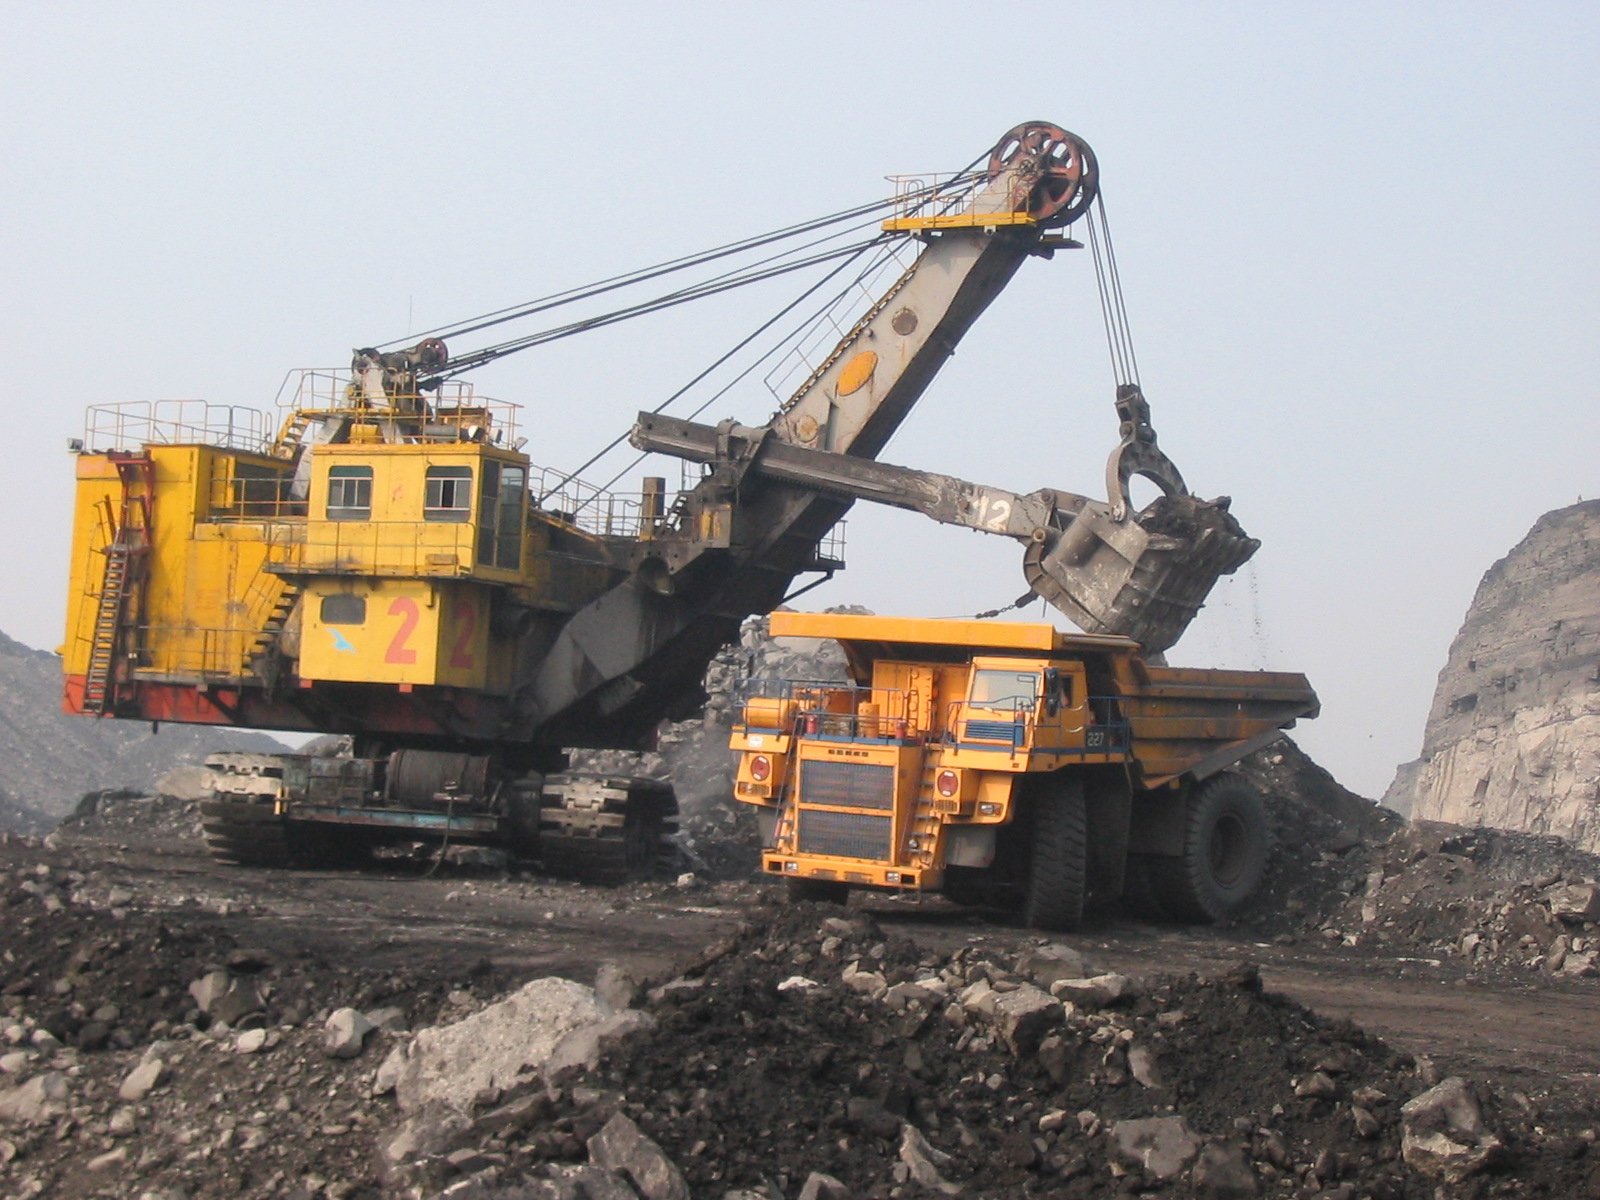
\includegraphics[width=.6\linewidth]{Exc/Excavator} \\
		\tiny{originally posted to Flickr by FAndrey at http://flickr.com/photos/43301444@N06/4141786255}
	\end{figure}

	\begin{itemize}
		\item{Goal: \textbf{optimization of model parameters}}
		\item{Models of technical system = physical properties + control properties}
	\end{itemize}
\end{frame}

\begin{frame}
	\frametitle{Problem Setting}
	\begin{figure}[bth]
		\centering
		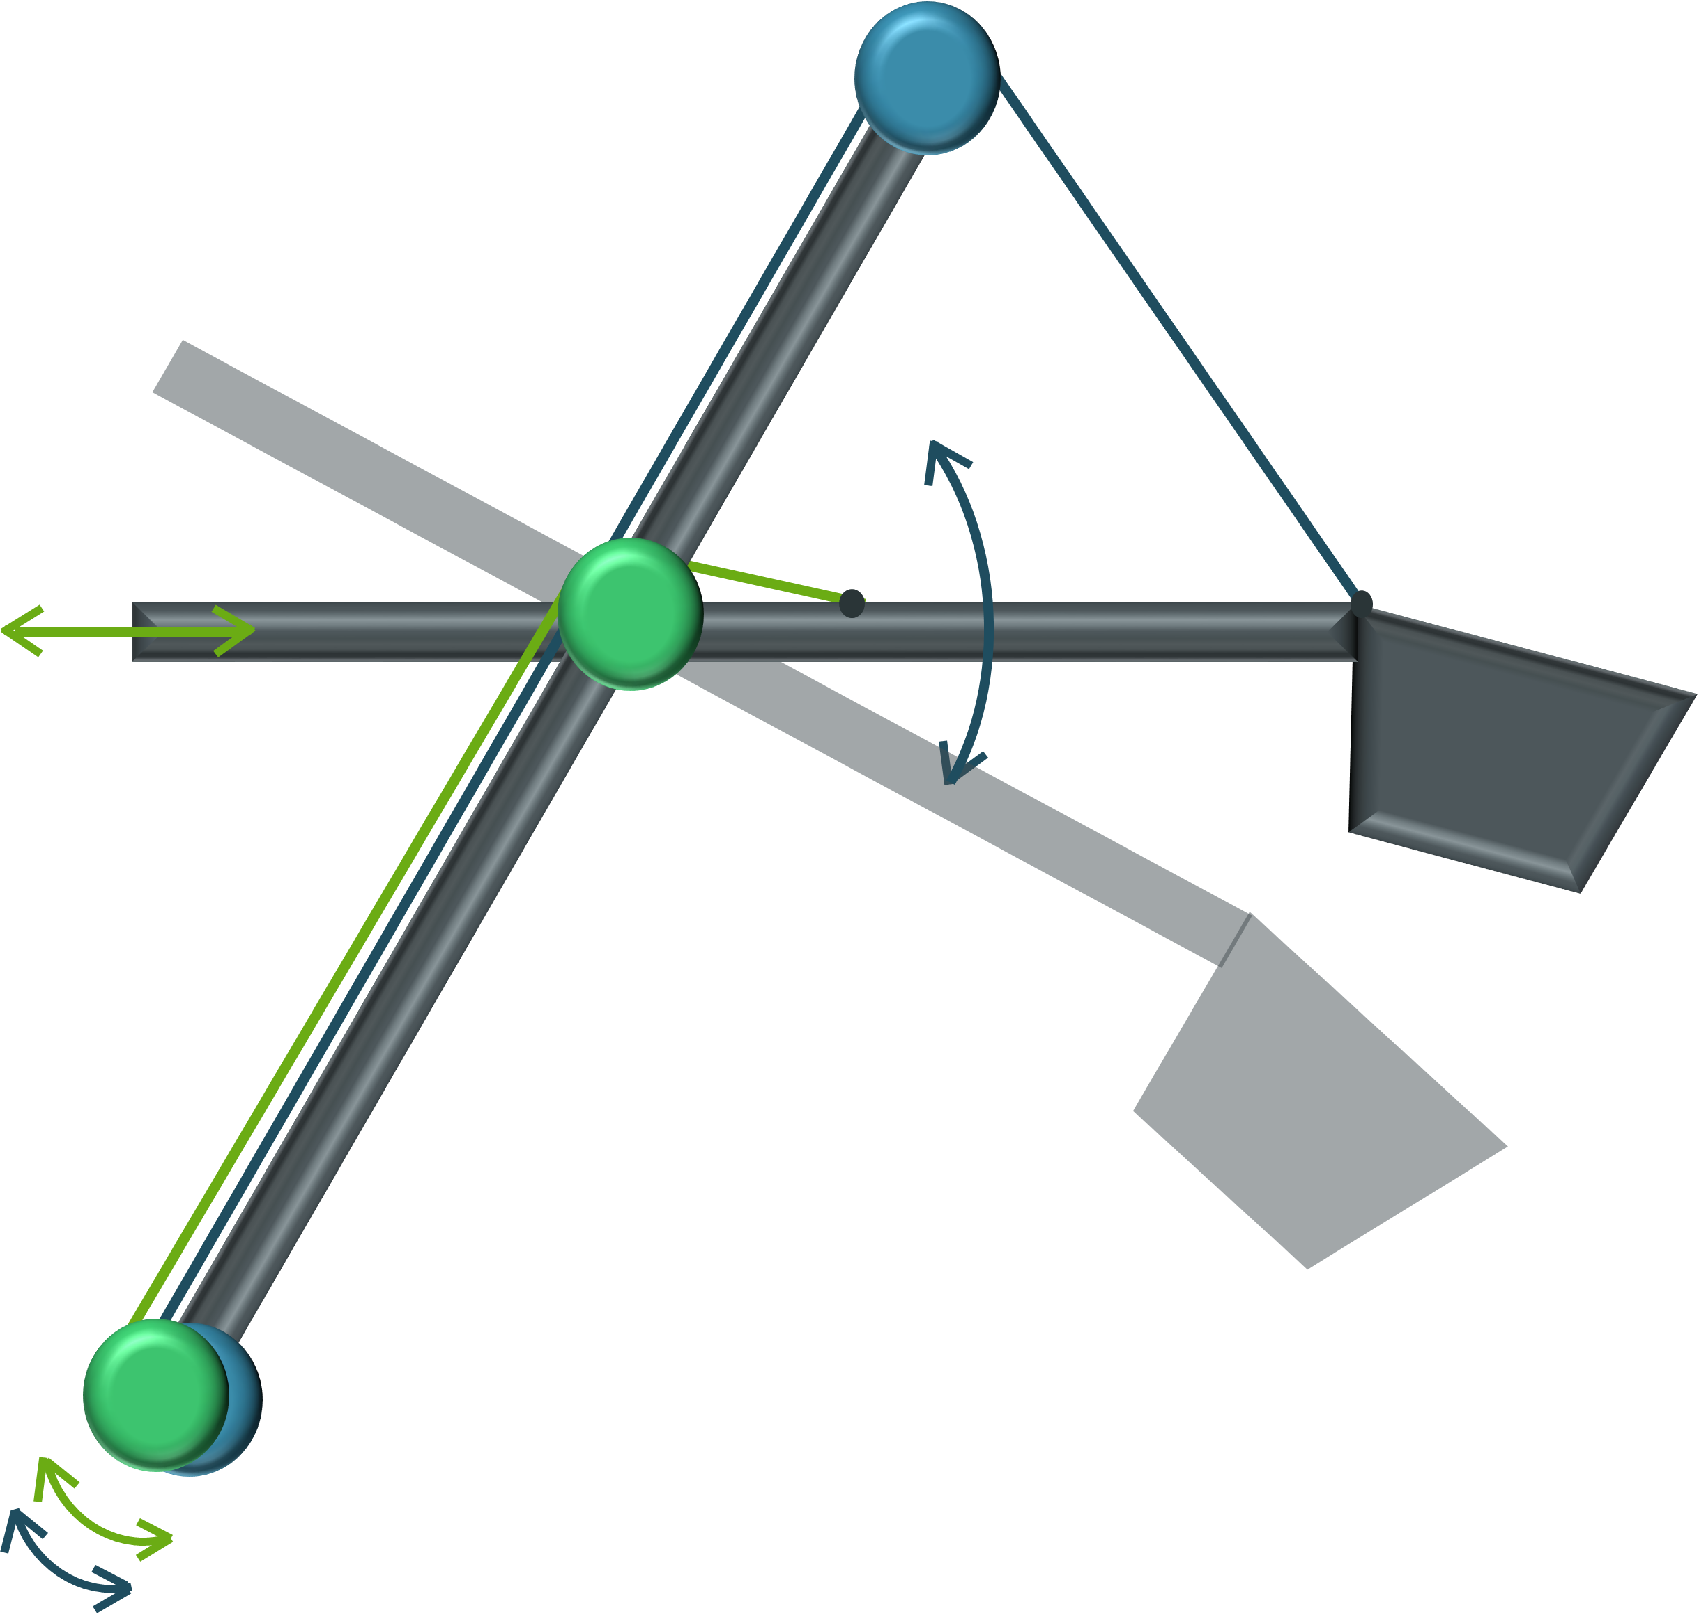
\includegraphics[width=0.4\linewidth]{Exc/Problem_1}
	\end{figure}
\end{frame}

\begin{frame}
	\frametitle{Problem Setting}
	\begin{figure}[bth]
		\centering
		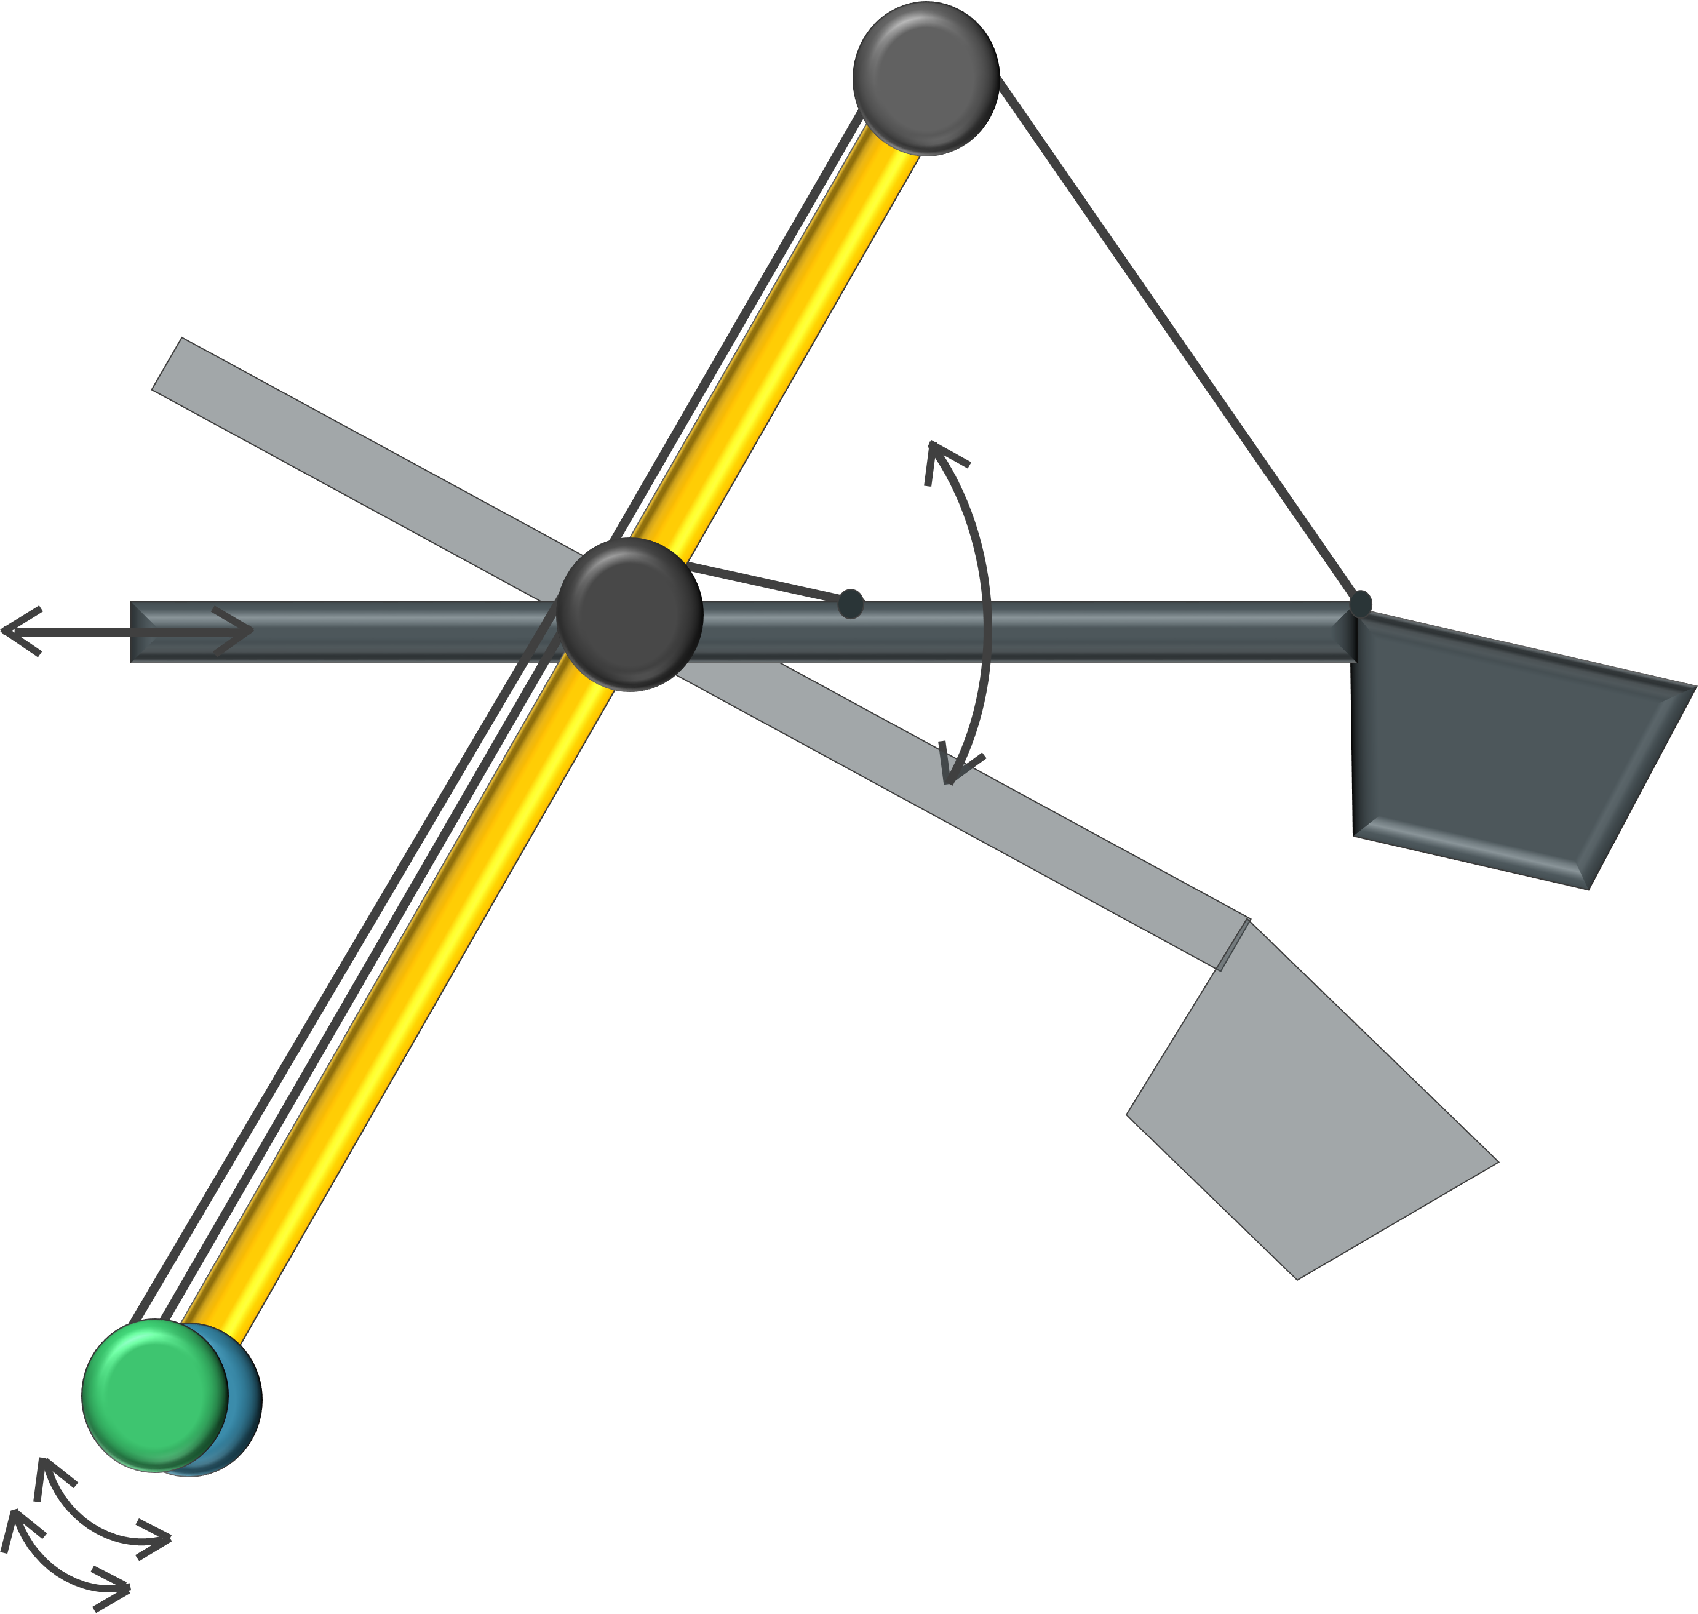
\includegraphics[width=0.4\linewidth]{Exc/Problem_2}
	\end{figure}
	\begin{itemize}
		\item{arm element fixed to base}
		\item{cannot be moved w.r.t. the base}
	\end{itemize}
\end{frame}

\begin{frame}
	\frametitle{Problem Setting}
	\begin{figure}[bth]
		\centering
		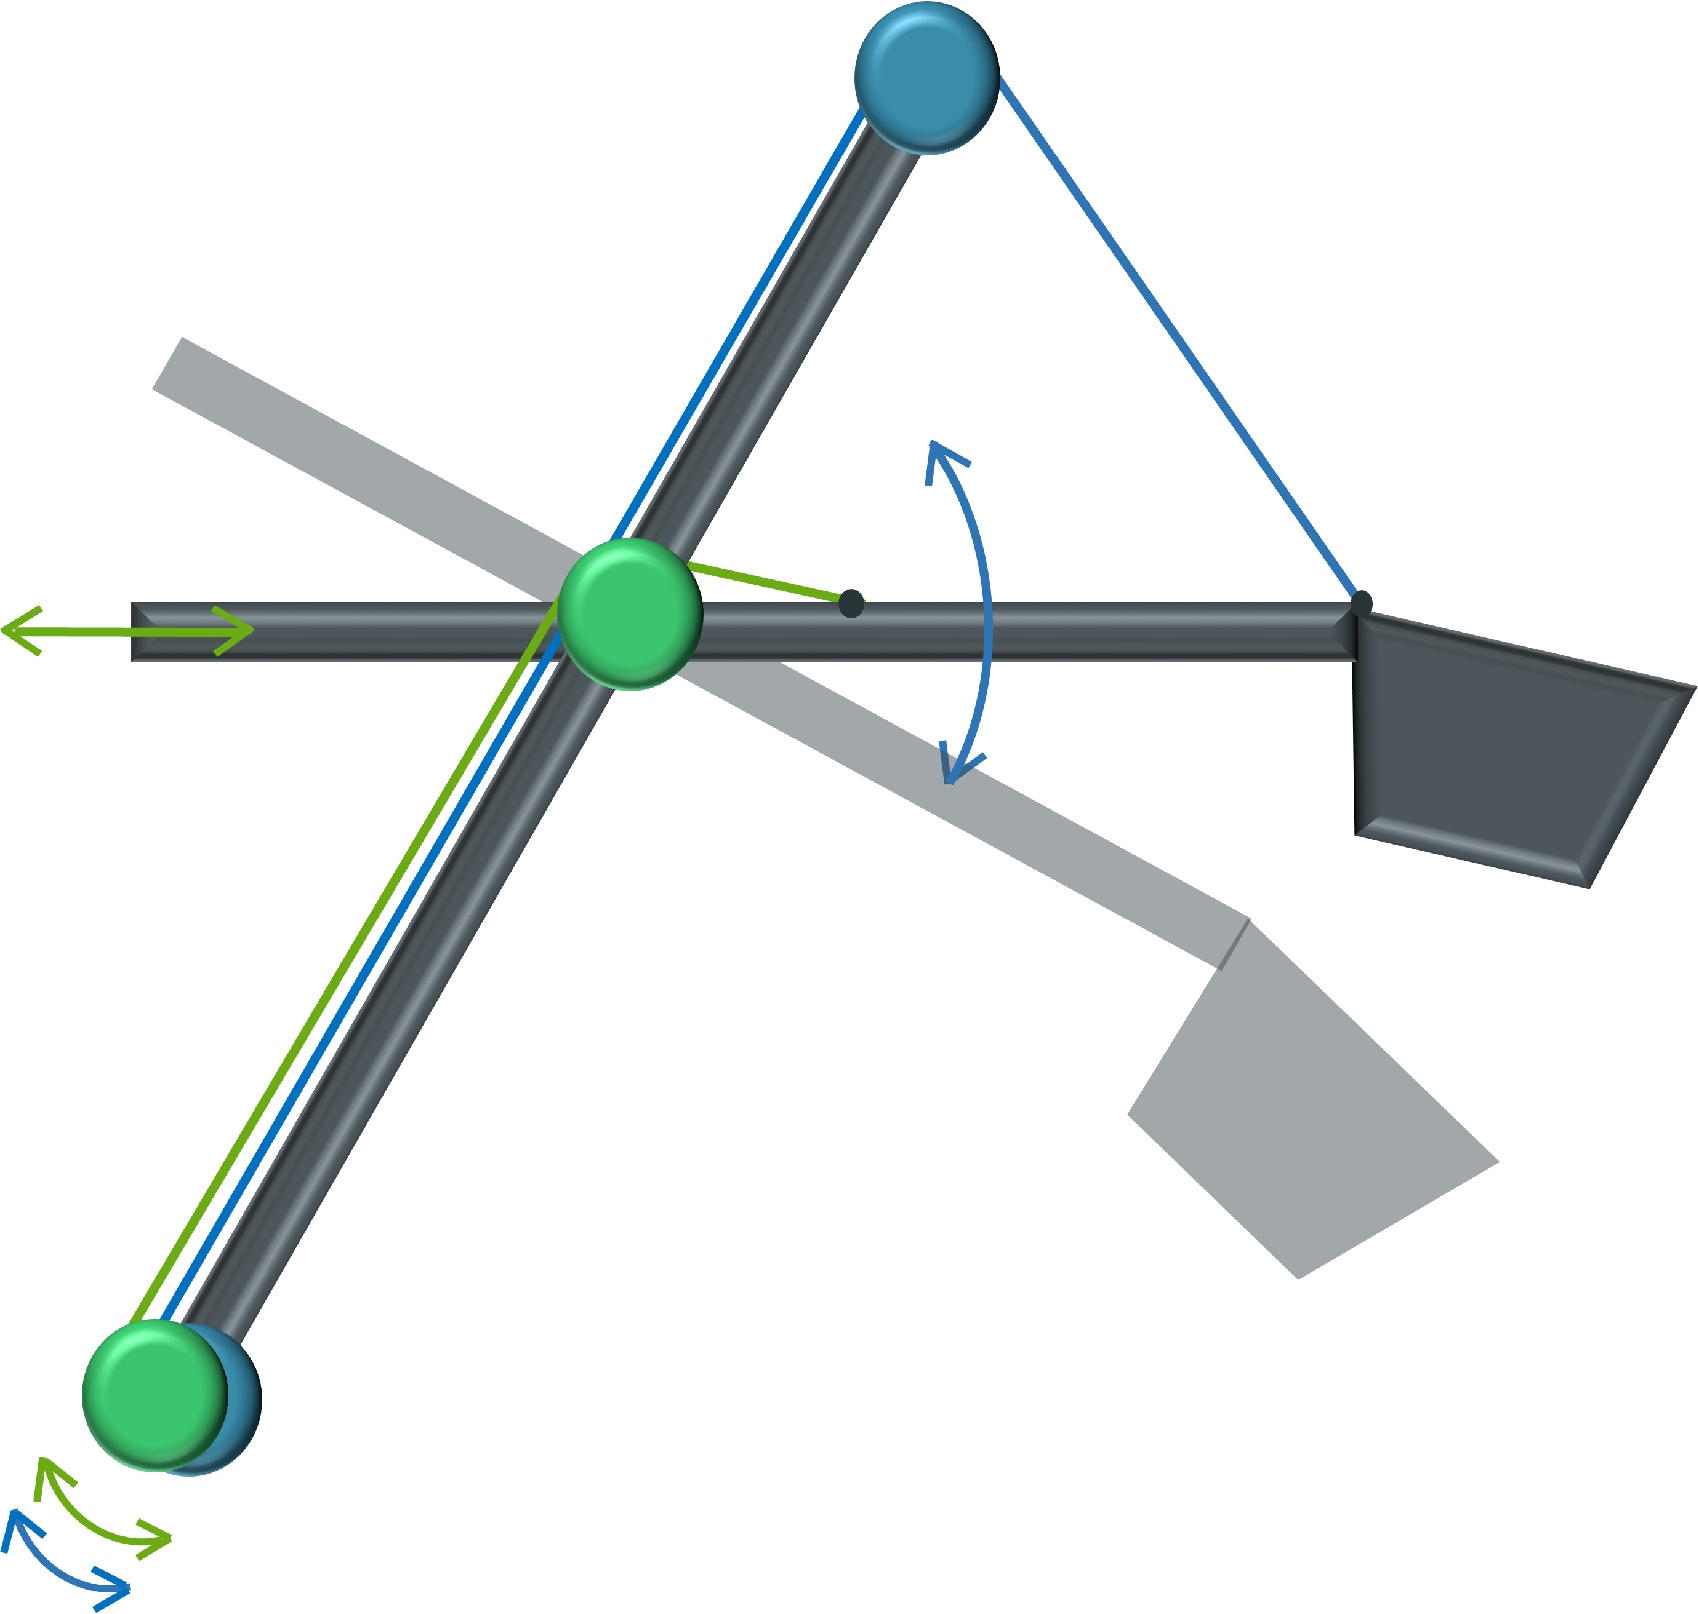
\includegraphics[width=0.4\linewidth]{Exc/Problem_3}
	\end{figure}
	\centering
	\begin{tabular}{ll}
		\textcolor[rgb]{0,0.69,0.32}{green} & shovel motion \textbf{back} and \textbf{forth} \\
		\textcolor[rgb]{0.18,0.46,0.71}{blue} & shovel motion \textbf{up} and \textbf{down} \\
	\end{tabular}
\end{frame}

\begin{frame}[c]
	\frametitle{Main Problems}
	\begin{enumerate}
		\item{Phyiscal Modelling}
			\begin{itemize}
				\item{modelling rope properties}
				\item{determining information needed for calibration of model}
			\end{itemize}
		\vspace{0.5cm}
		\item{Parameter Optimization}
			\begin{itemize}
				\item{optimizing parameters for a complex, unknown model (black box)}
			\end{itemize}
	\end{enumerate}
\end{frame}

\begin{frame}[c]
	\frametitle{Physical Modelling}
	Why?
	
	\vspace{0.5cm}
	
	\begin{columns}[t]
		\column{.3\linewidth}
			\centering
			\fbox{\parbox{\textwidth}{building an accurate model}}
		\column{.2\linewidth}
			\centering
			$\Rightarrow$
		\column{.3\linewidth}
			\centering
			\fbox{\parbox{\textwidth}{better visualization of control and motion}}
	\end{columns}
	
	\vspace{0.5cm}
	
	to consider:
	\begin{itemize}
		\item{friction in cable reels}
		\item{deformation of ropes}
	\end{itemize}
\end{frame}

\begin{frame}[c]
	\frametitle{Parameter Optimization}
	What are parameters?
	\begin{itemize}
		\item{friction coefficients}
		\item{mass}
		\item{inertia}
	\end{itemize}
	
	\vspace{0.5cm}
	
	Why?
	
	\vspace{0.5cm}
	
	\begin{columns}
		\column{.3\textwidth}
			\centering
			\fbox{\parbox{\textwidth}{accurate and realistic parameters}}
		\column{.2\textwidth}
			\centering
			$\Rightarrow$
		\column{.3\textwidth}
			\fbox{\parbox{\textwidth}{better prediction and planning of motion}}
	\end{columns}
\end{frame}

%------------------------------------------------------------------------- Physikal Model --------------------------------------------------------------------------------

\section{Physical Model}

\begin{frame}
	\frametitle{Involved Forces}
	\begin{figure}[bth]
	  \begin{center}
	    %left, bottom, right, top
	    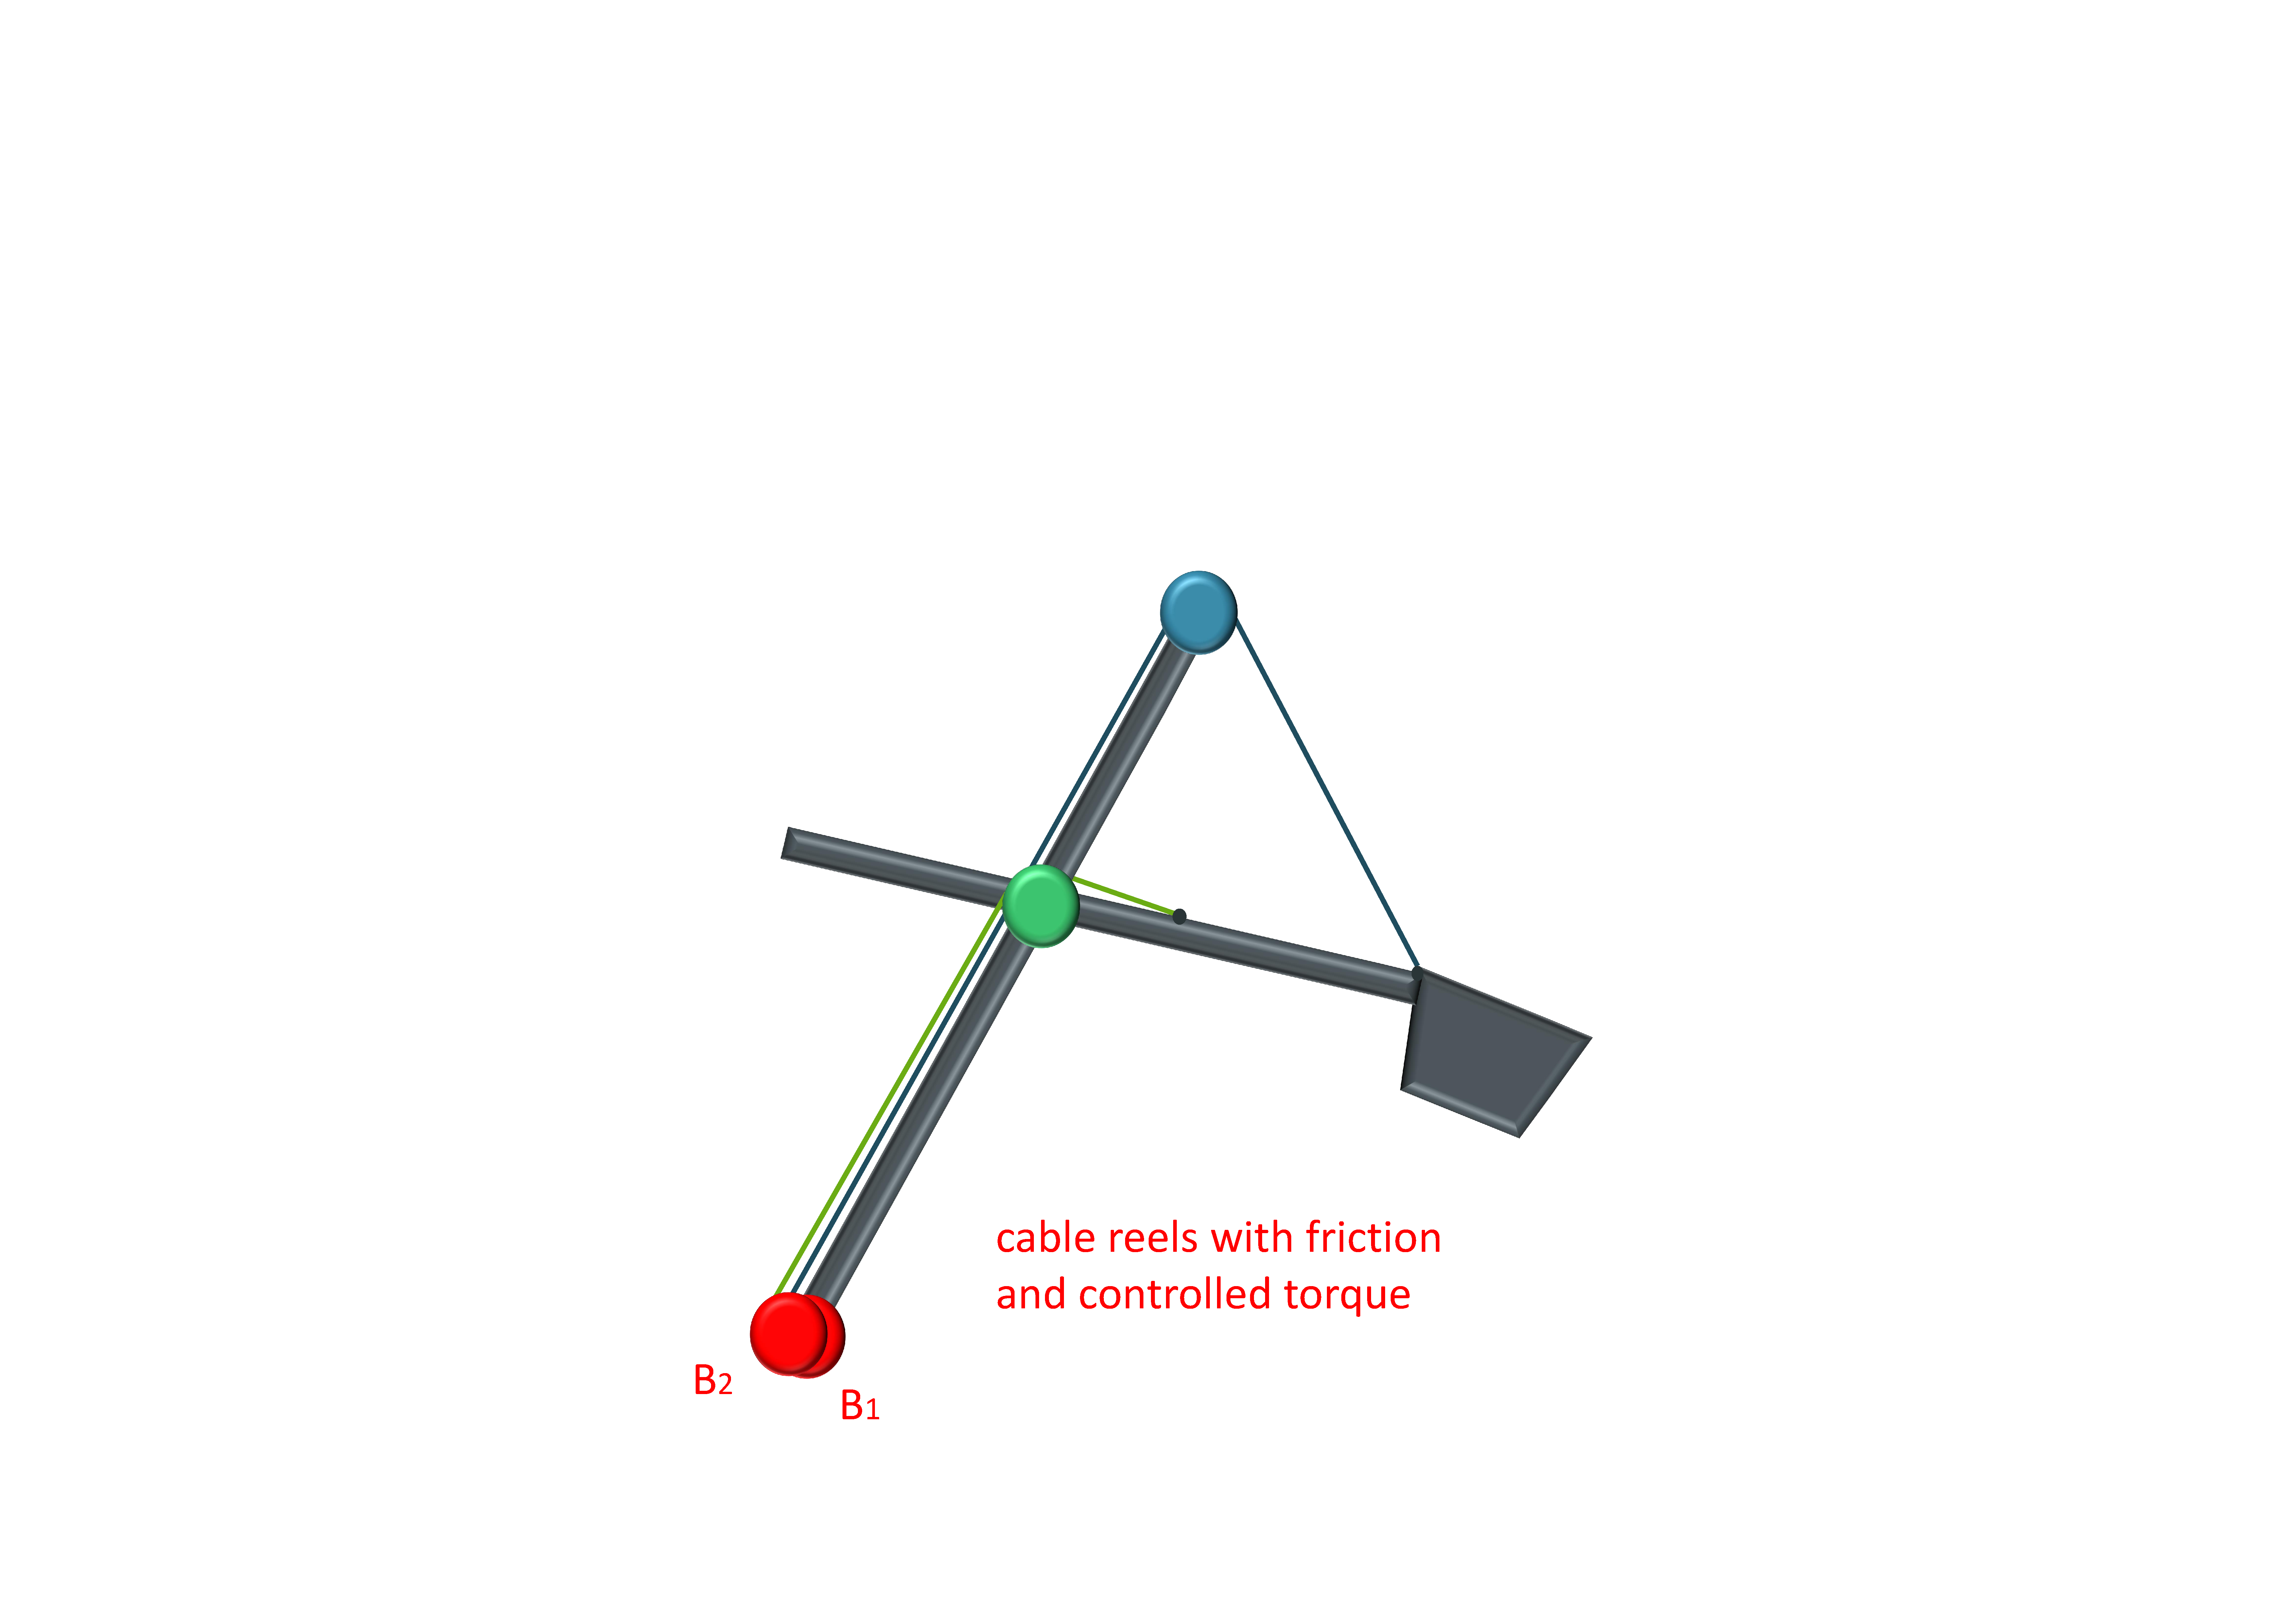
\includegraphics[trim=22cm 5cm 2cm 24cm, clip=true, 
	    width=\linewidth]{Exc/Excavator_Only1}
	  \end{center}
	\end{figure}

\end{frame}

\begin{frame}
	\frametitle{Involved Forces}
	
	\begin{figure}[bth]
	  \begin{center}
	    %left, bottom, right, top
	    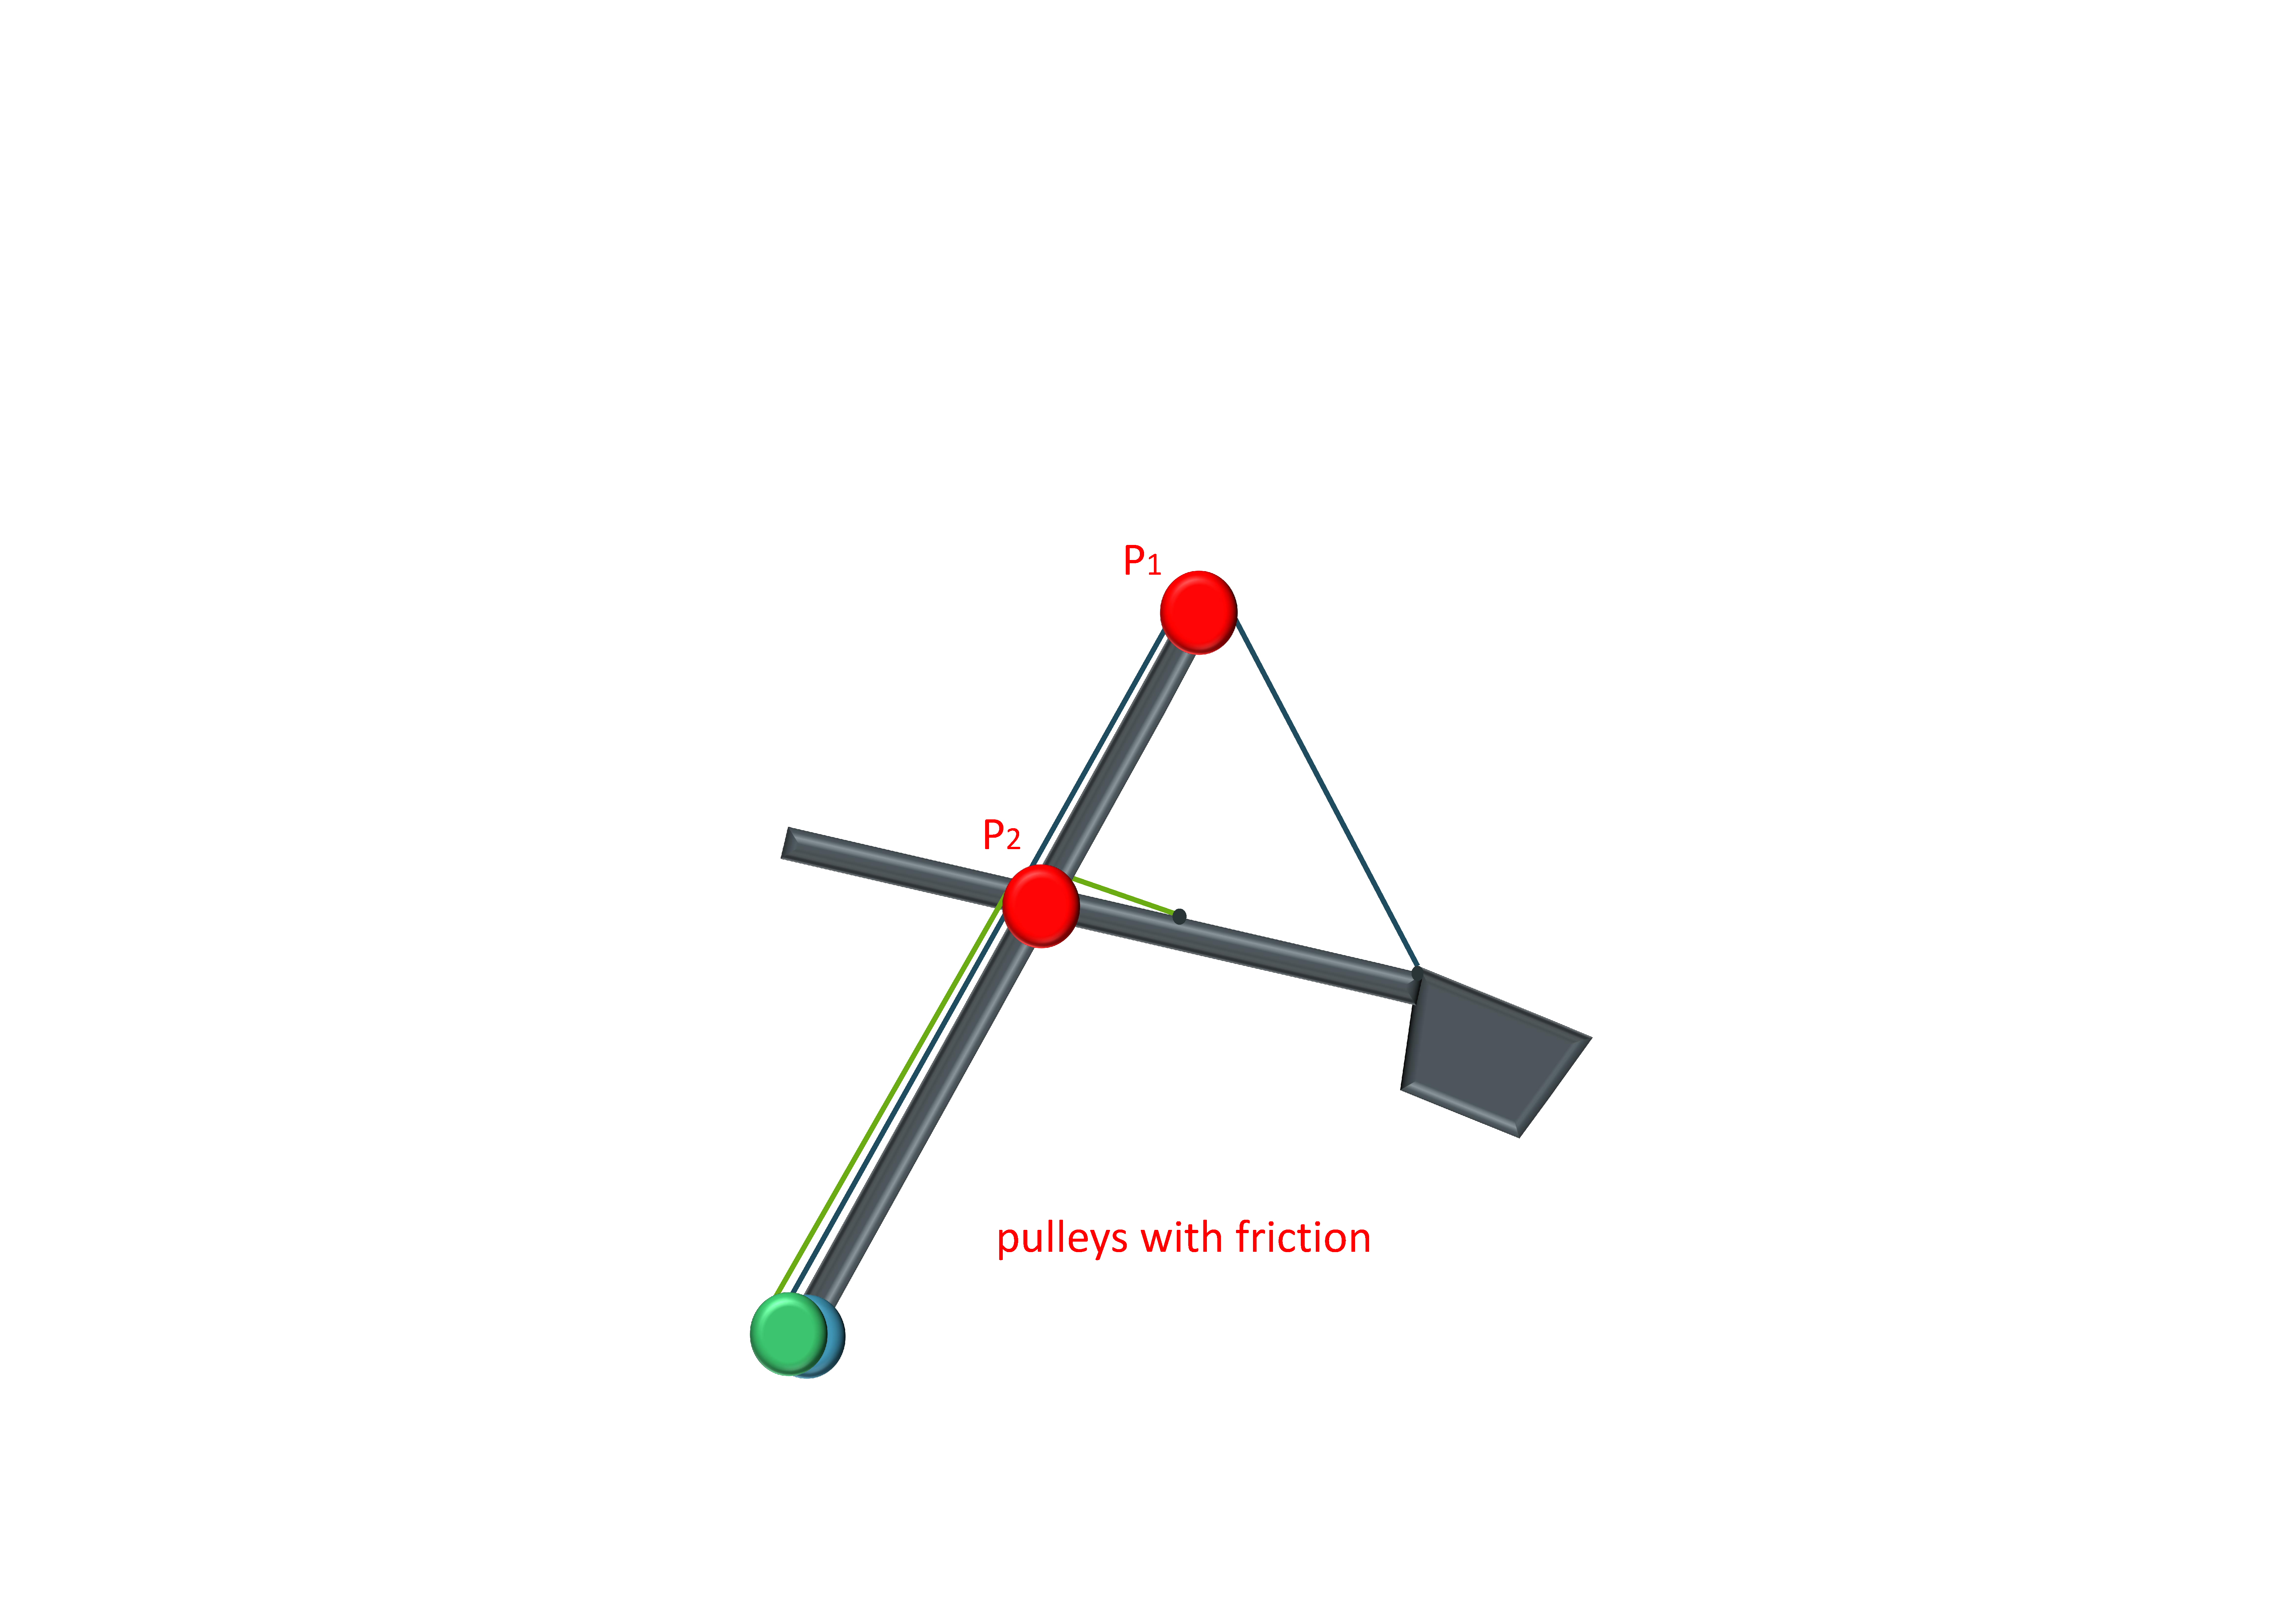
\includegraphics[trim=22cm 5cm 2cm 24cm, clip=true, 
	    width=\linewidth]{Exc/Excavator_Only2}
	  \end{center}
	\end{figure}

\end{frame}

\begin{frame}
	\frametitle{Involved Forces}
	
	\begin{figure}[bth]
	  \begin{center}
	    %left, bottom, right, top
	    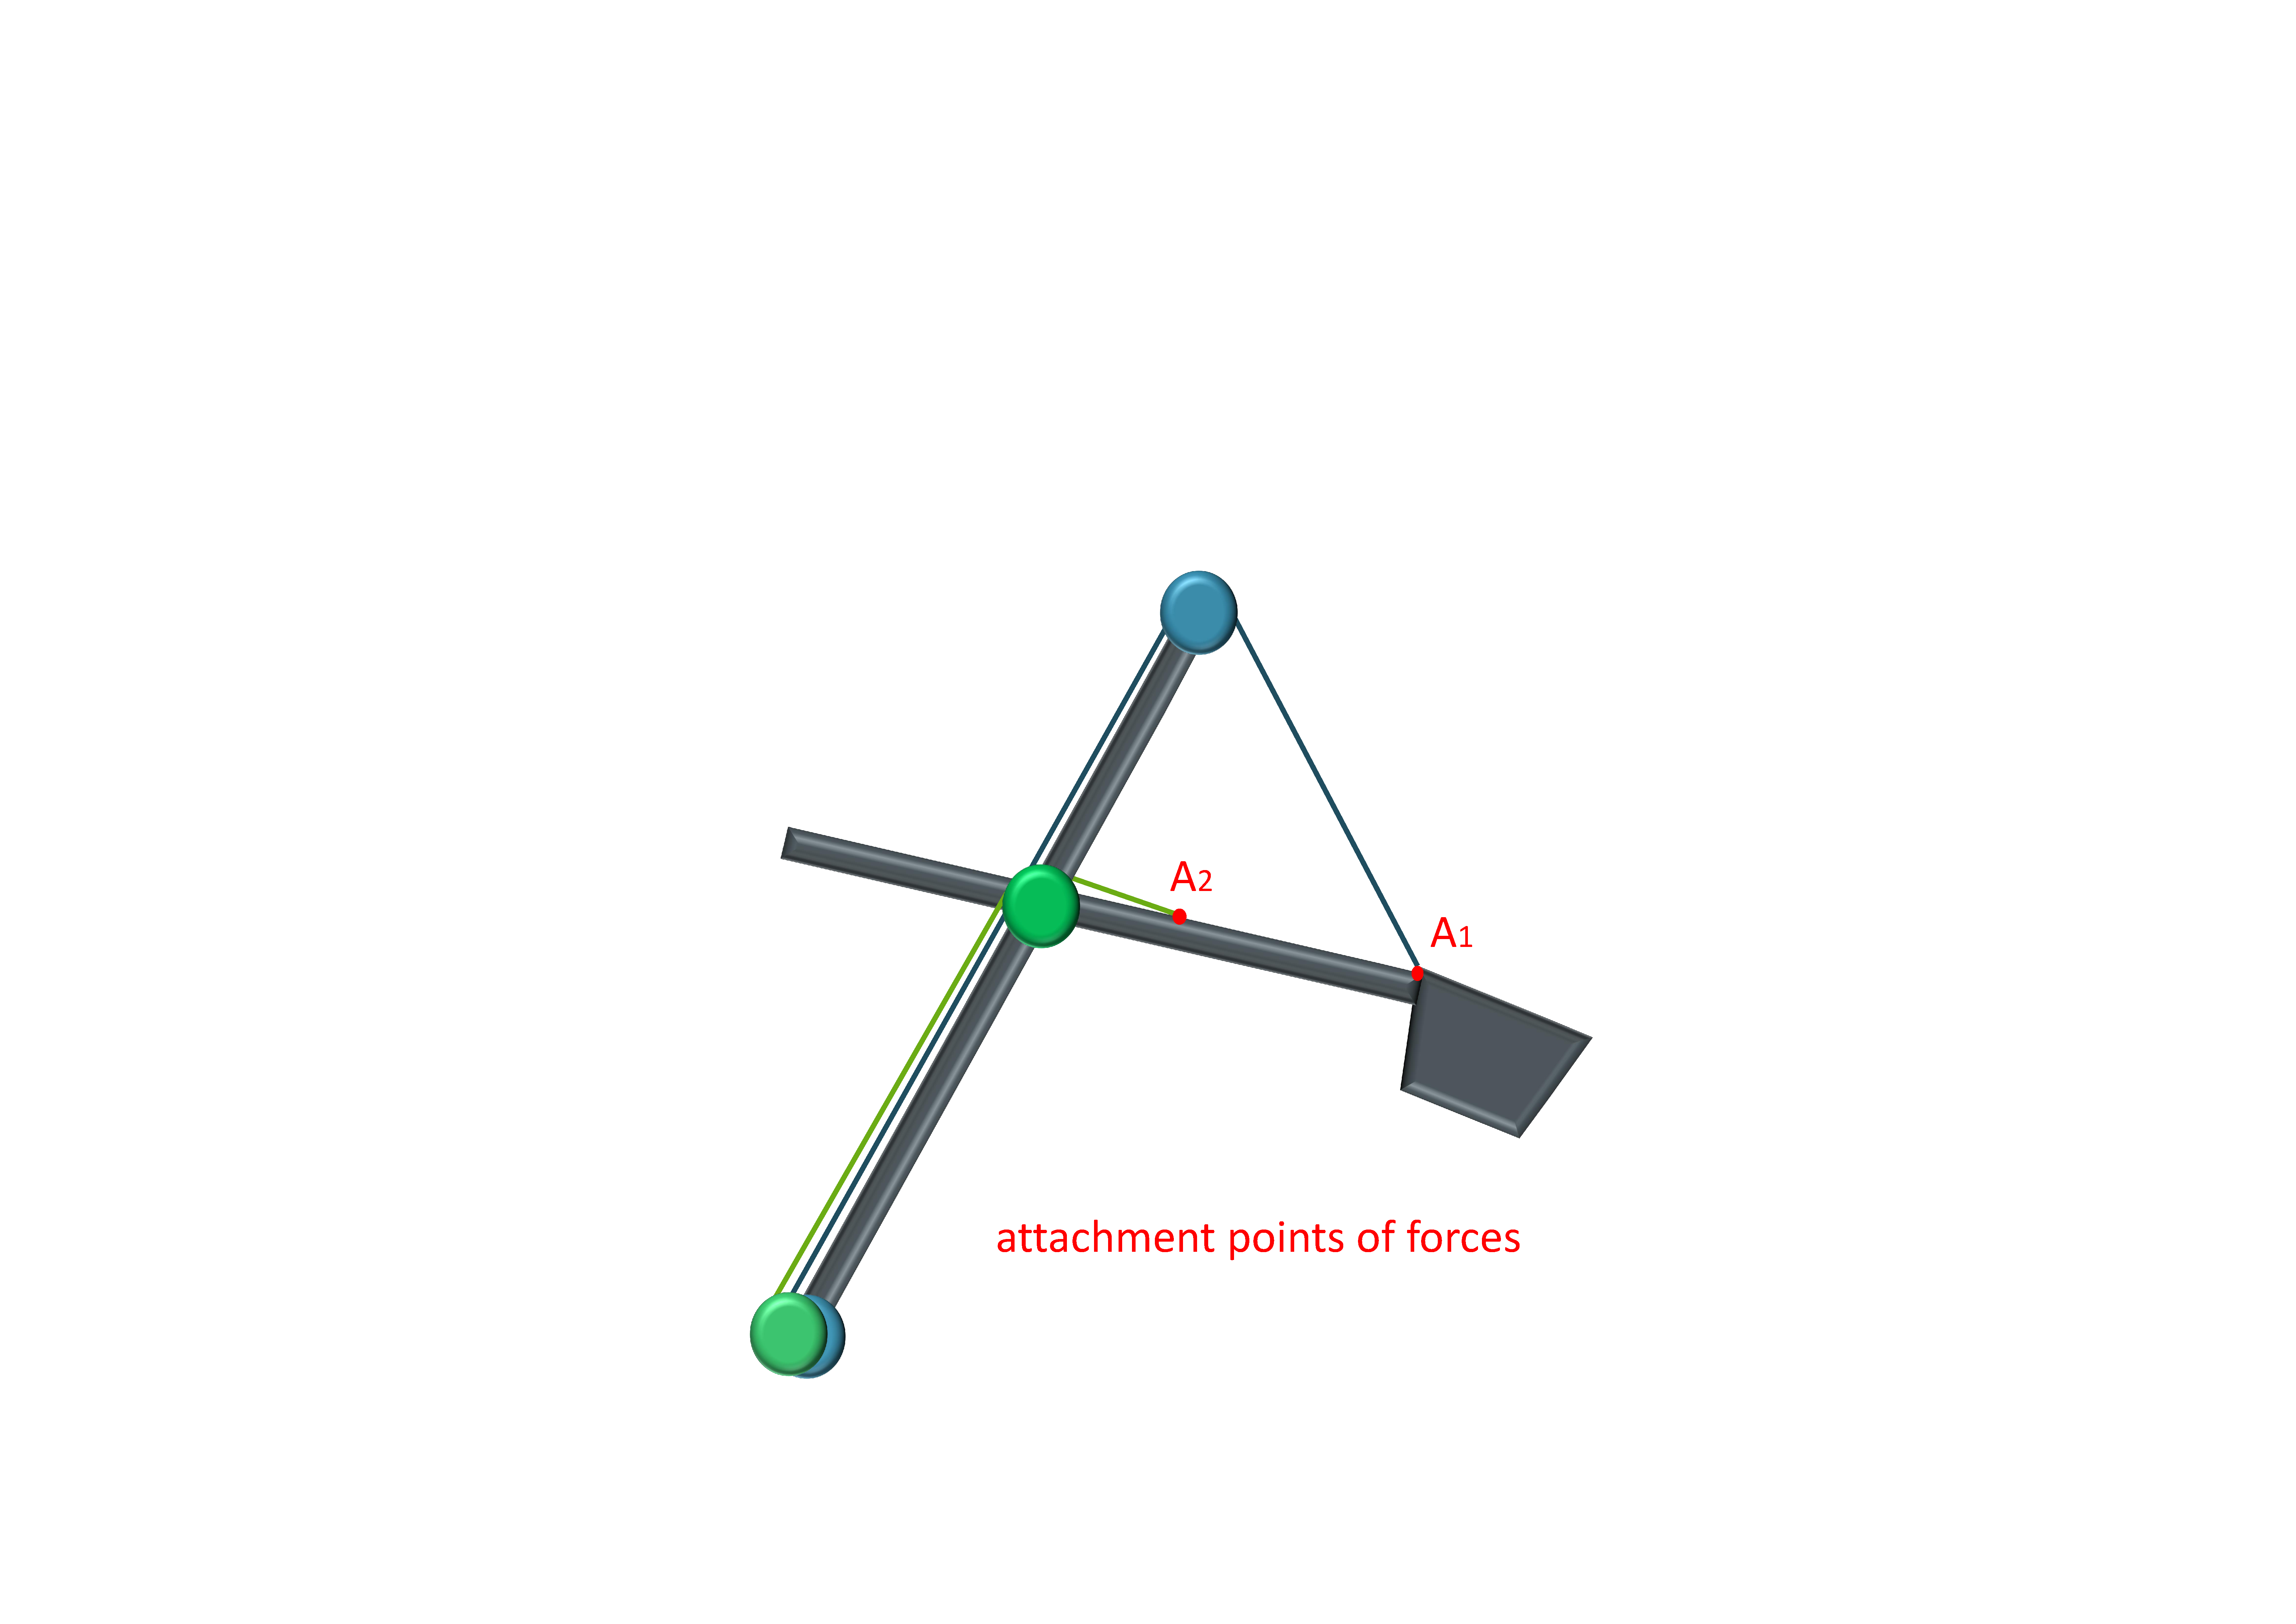
\includegraphics[trim=22cm 5cm 2cm 24cm, clip=true, 
	    width=\linewidth]{Exc/Excavator_Only3}
	  \end{center}
	\end{figure}

\end{frame}

\begin{frame}
	\frametitle{Generalized Forces Q}
	
	Example: force at $A_2$:
	\begin{align*}
	  &F_{A_2} = \left[ \frac{\tau_{B_2}}{r_{B_2}} - \mu_{B_2} 
	  \frac{\dot{s}}{r_{B_2}} - \mu_{P_2} \frac{\dot{s}}{r_{P_2}} \right]
	  \left(
	  \begin{matrix}
	    \cos(\theta) \\
	    \sin(\theta) \\
	  \end{matrix}
	  \right) \\
	\end{align*}
	
	all generalized forces:
	\begin{align*}
	  &Q_s = \left( \frac{\partial r_{A_1}}{\partial s} \right)^T F_{A_1} 
	  + \left( \frac{\partial r_{A_2}}{\partial s} \right)^T F_{A_2} \\
	  &Q_{\theta} = \left( \frac{\partial r_{A_1}}{\partial \theta} 
	  \right)^T F_{A_1} + \left( \frac{\partial r_{A_2}}{\partial \theta} 
	  \right)^T F_{A_2} \\
	\end{align*}
\end{frame}

\begin{frame}
	\frametitle{Parameters}
	
	\begin{tabular}{ll}
	  & \\
	  masses & $M_1$, $M_2$ \\
	  &\\
	  inertia of pulleys & $I_{B_1}$, $I_{B_2}$, $I_{P_1}$, $I_{P_2}$ \\
	  &\\
	  friction coefficients & $\mu_{B_1}$, $\mu_{B_2}$, $\mu_{P_1}$, 
	  $\mu_{P_2}$  \\
	\end{tabular}
\end{frame}

\begin{frame}
	\frametitle{Lagrangean Formalism}
	
	\begin{align*}
	  &\frac{d}{dt}\left(\frac{\partial T}{\partial \dot{s}}\right) -
	  \frac{\partial T}{\partial s} +
	  \frac{\partial V}{\partial s}
	  = Q_s \\
	  &{}\\
	  &\frac{d}{dt}\left(\frac{\partial T}{\partial \dot{\theta}}\right) -
	  \frac{\partial T}{\partial \theta} +
	  \frac{\partial V}{\partial \theta}
	  = Q_{\theta} \\
	\end{align*}
\end{frame}

\begin{frame}[c]
	\frametitle{Resulting ODE}
	
	Second order ODE from Lagrange formalism:
	\begin{align*}
	  &A(x,p)
	  \begin{pmatrix} 
	    \ddot{s} \\ \ddot{\theta} \\
	  \end{pmatrix}
	  = b(x,u,p)
	\end{align*}
	
	T	ransformed into first order ODE:
	\begin{align*}
	  &\frac{d}{dt}
	  \begin{pmatrix}
	  s \\ \theta \\ \dot{s} \\ \dot{\theta}
	  \end{pmatrix}
	  =
	  \begin{pmatrix}
	    \dot{s} \\ \dot{\theta} \\ A^{-1}(x,p)b(x,u,p) \\
	  \end{pmatrix} 
	  = f(x,u,p) \\
	\end{align*}
	
	\vspace{-1.0cm}
	
	\begin{tabular}{ll}
	  & \\
	  state & $ x = (s,\theta,\dot{s},\dot{\theta})^T $ \\
	  control & $ u = (\tau_1,\tau_2)^T $ \\
	  parameters & $ p = (p_1,...,p_k)^T $ \\
	\end{tabular}
\end{frame}

\begin{frame}
	\frametitle{Discretization of the ODE}
	
	Discretize time interval:
	\begin{align*}
	  &[0,T] = [t_0,t_1] \cup \ldots \cup [t_{m-1},t_m] \\
	\end{align*}
	
	Discretize state and control:
	\begin{align*}
	  &x_n = x(t_n) \\
	  &u_n = u(t_n) \\
	\end{align*}
	
	Solve ODE for every time step $h_n=t_{n+1}-t_n$ (Forward Euler):
	\begin{align*}
	  &\tilde{x}_{n+1} = x_n + h_n f(x_n,u_n,p) \\
	\end{align*}
\end{frame}

\begin{frame}
	\frametitle{Multiple Shooting}
	
	\begin{figure}[bth]
	  \begin{center}
	    %left, bottom, right, top
	    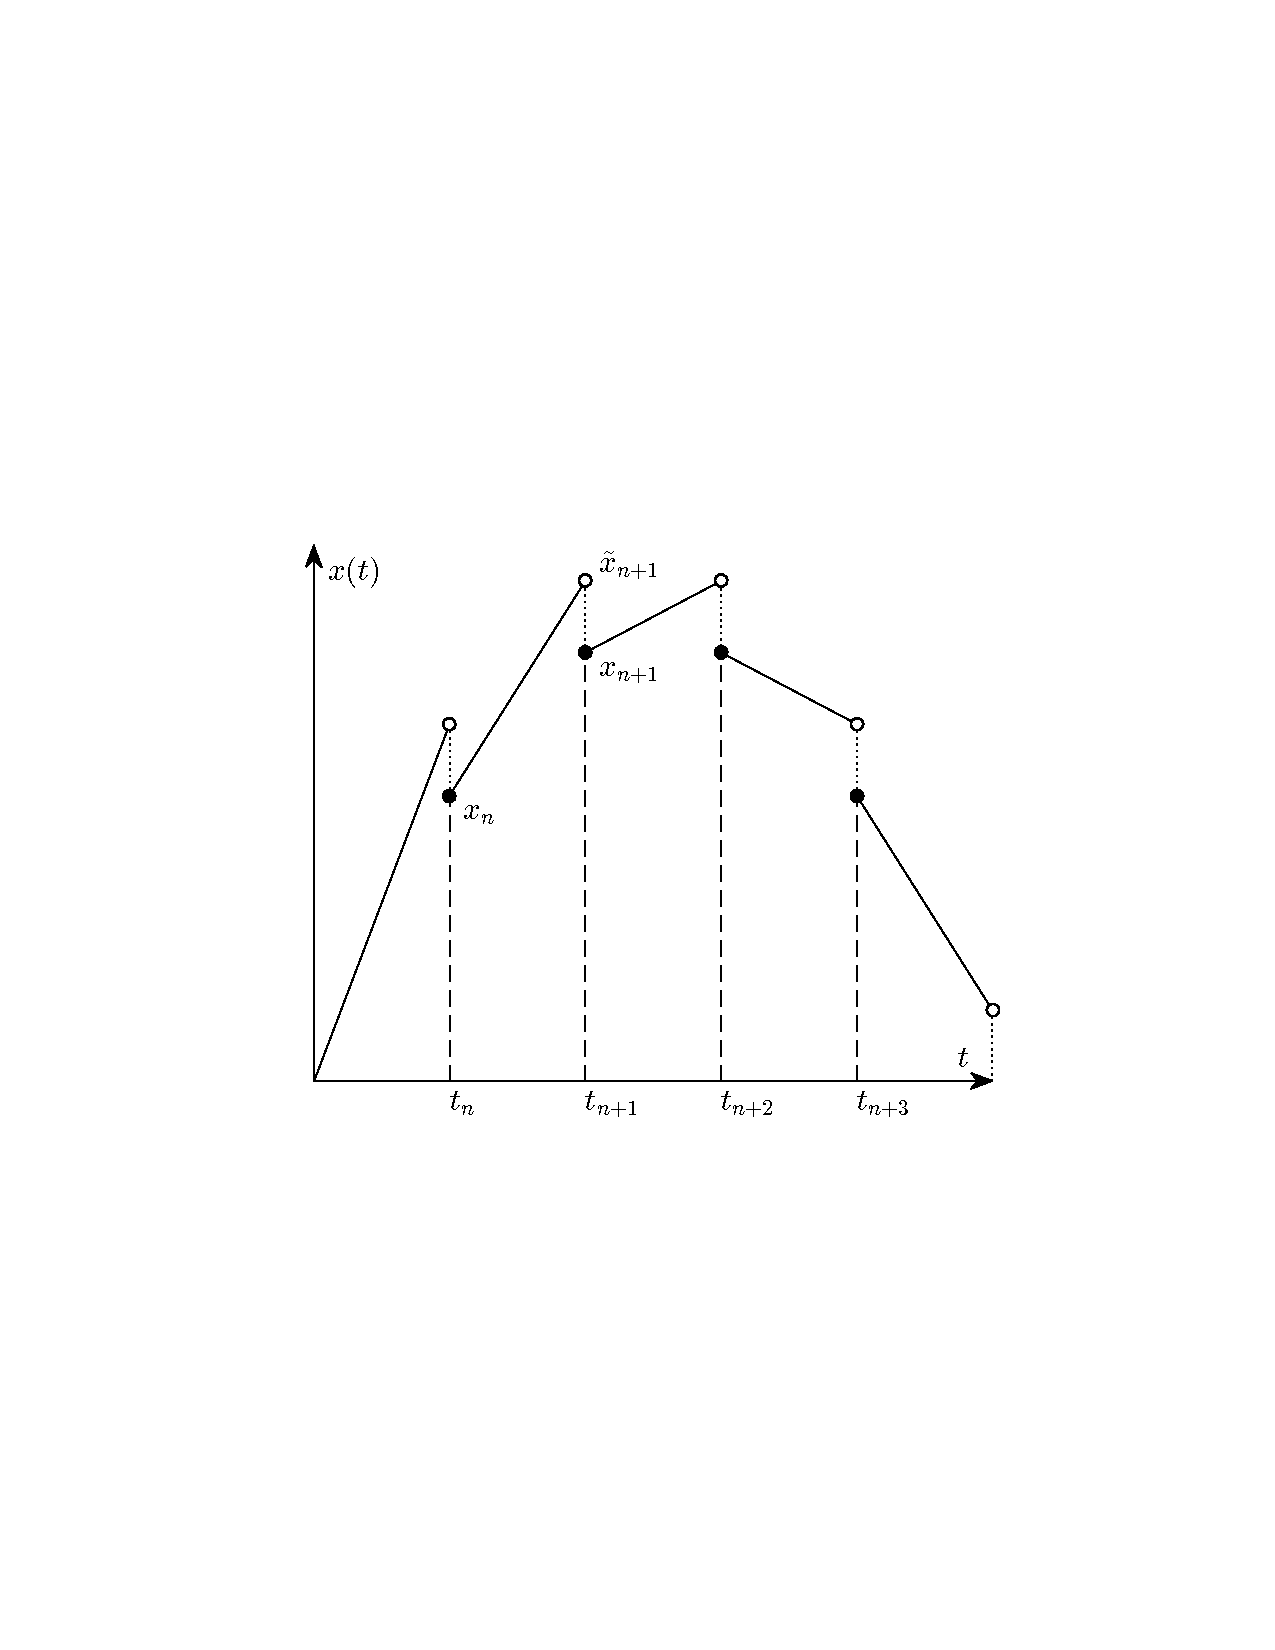
\includegraphics[trim=1cm 5cm 0cm 8cm, clip=true, 
	    width=\linewidth]{Exc/multShootPlot}
	  \end{center}
	\end{figure}
\end{frame}

\begin{frame}
	\frametitle{Lagrange Formalism}
	
	Method to describe dynamics of an accelerated system\\
	\begin{small}
	\begin{tabular}{ll}
		 & \\
		T & kinetic energy\\
		V & potentials\\
		F & non-conservative external forces\\
		r & vector pointing to origin of force F\\ %position vector
		q & free variables\\
		Q & generalized forces\\ \\
	\end{tabular}
	\end{small}
	\begin{align*}
	&\frac{d}{dt}\left(\frac{\partial T}{\partial \dot{q}_i}\right) -
	\frac{\partial T}{\partial q_i} +
	\frac{\partial V}{\partial q_i}
	= Q_i \\ \\
	& Q = \left(\frac{\partial r}{\partial q}\right)^T F\\
	\end{align*}
		
\end{frame}	

\begin{frame}
	\frametitle{Physical Model of Excavator}
	
	%left, bottom, right, top
	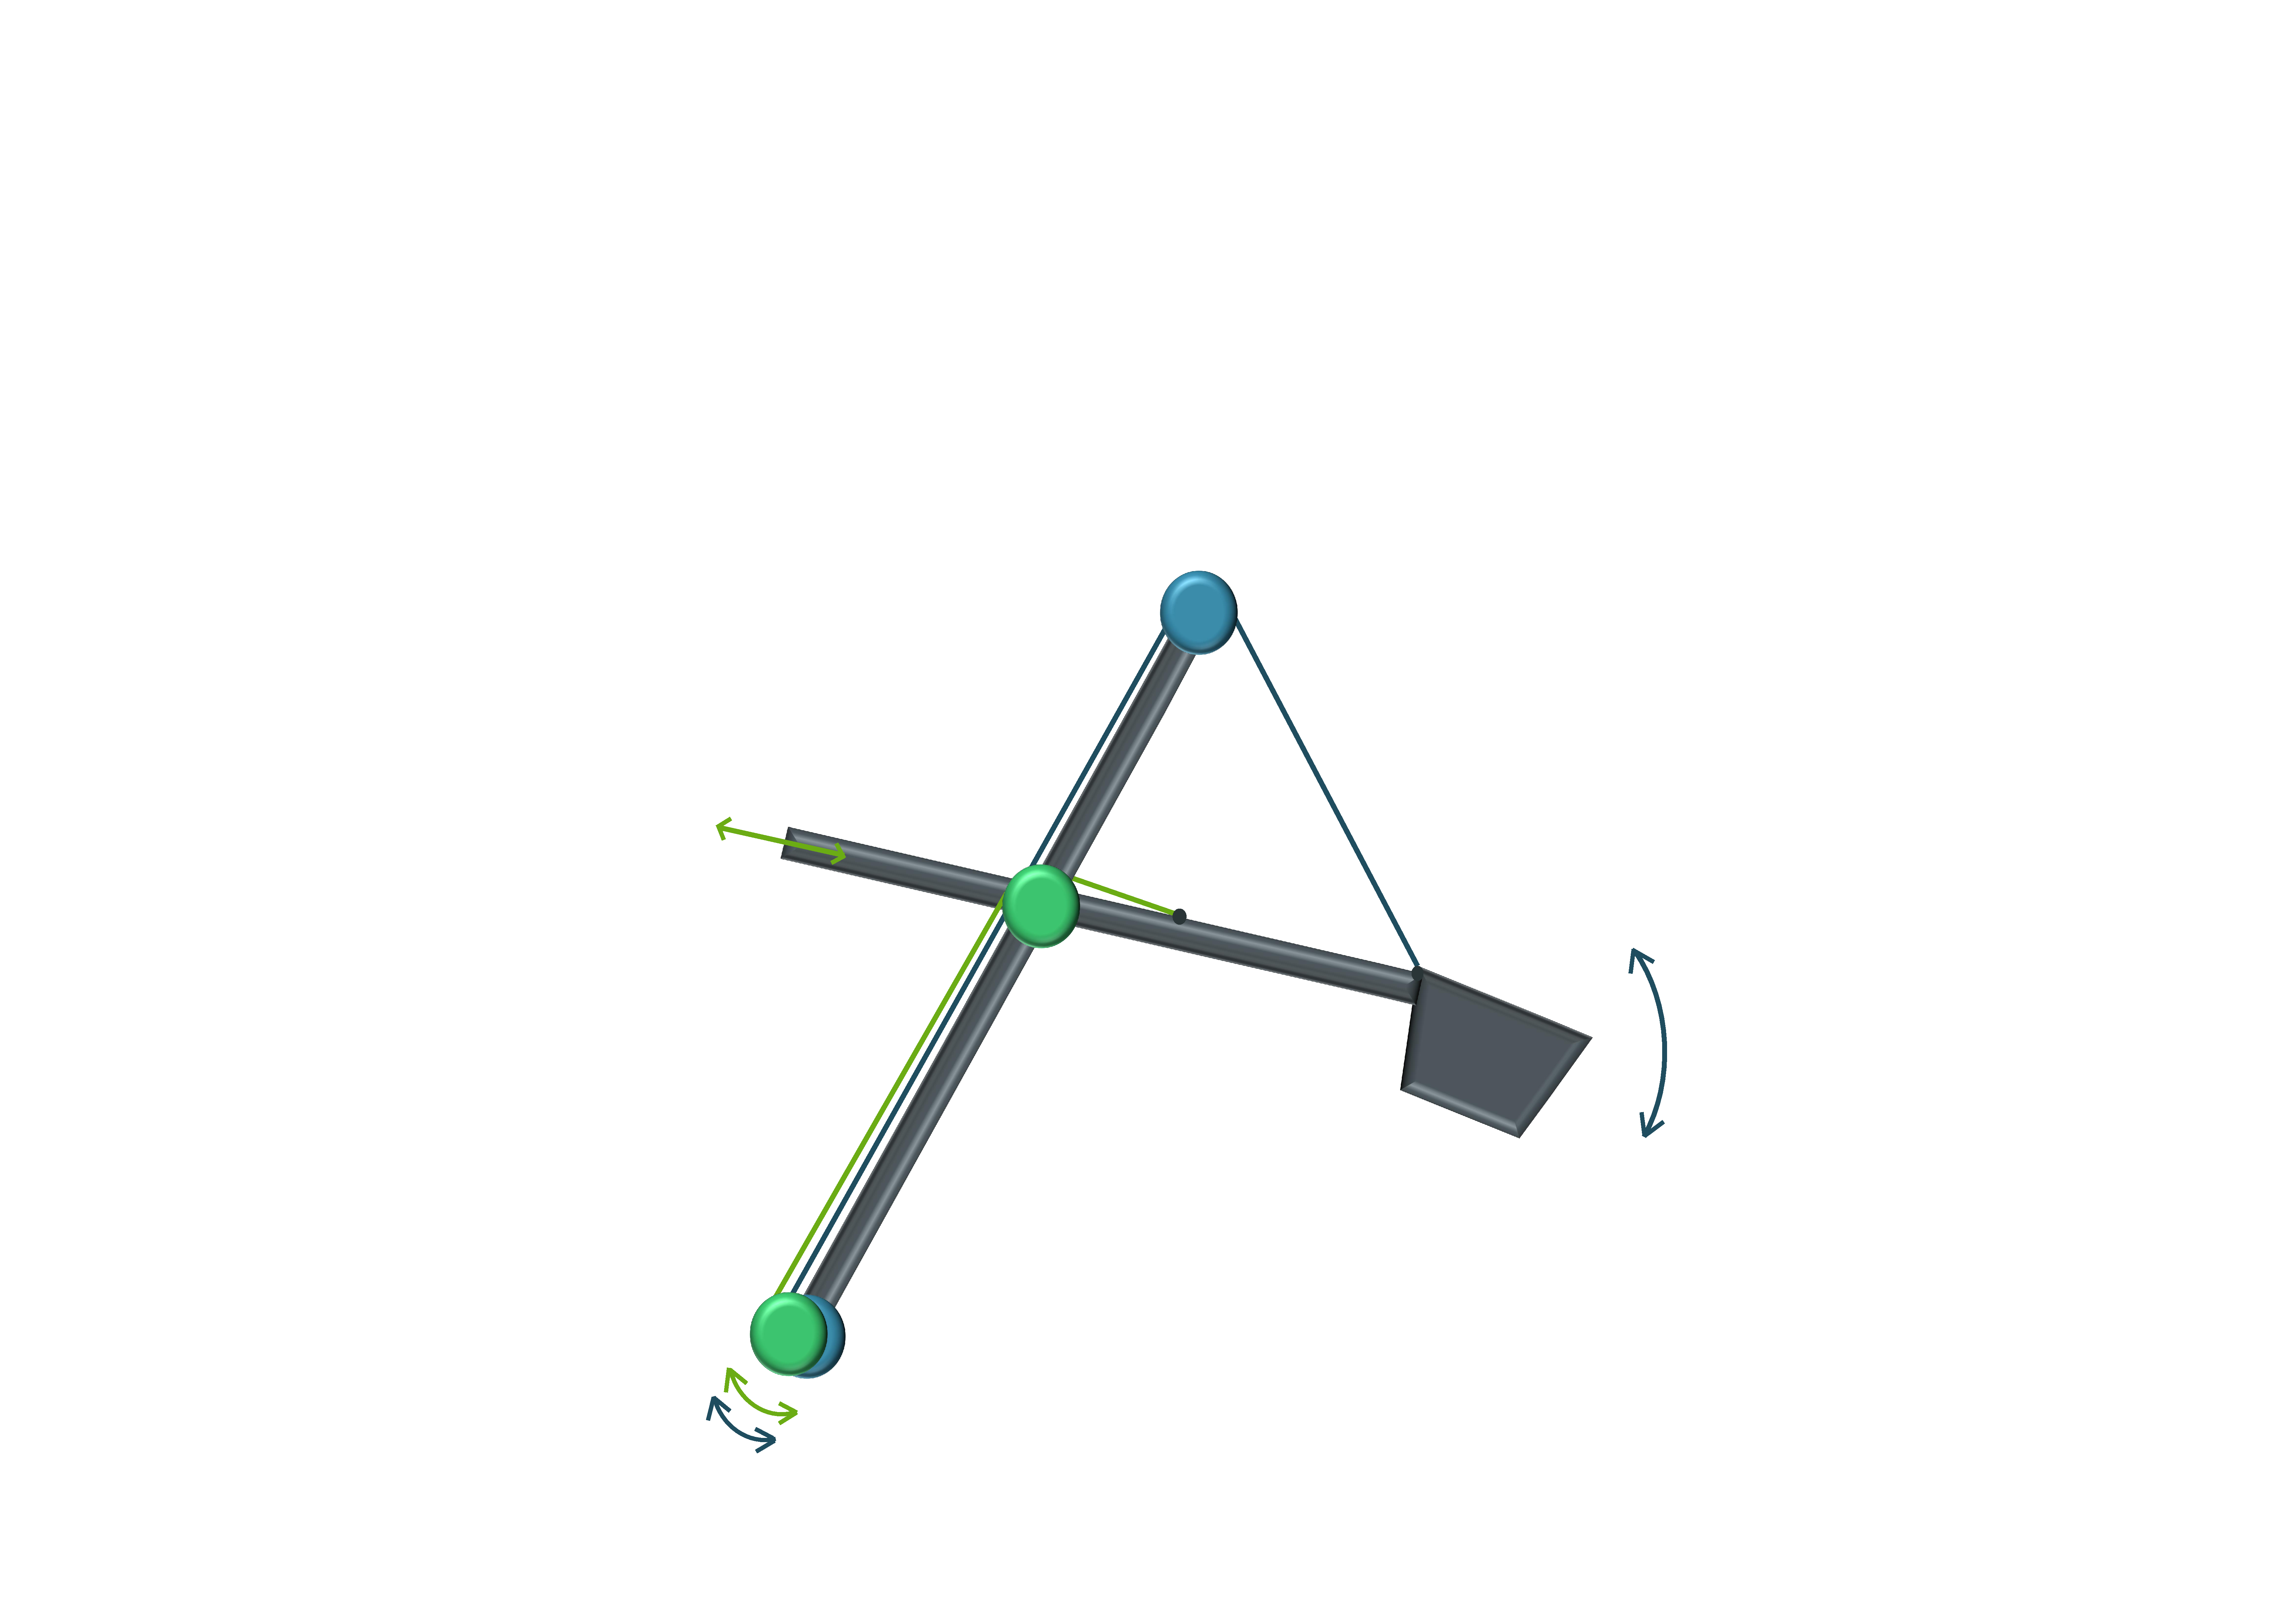
\includegraphics[trim=22cm 5cm 2cm 23cm, clip=true, width=\linewidth]{Exc/Excavator_Only}
	
\end{frame}

\begin{frame}
	\frametitle{Physical Model of Excavator}
	
	%	invariant under transformation of coordinates $\rightarrow$ appropriate choice of 	coordinate system
	
	%first fix coordinate system $\rightarrow$ consider positions vectors, coordinates of mass points,... in this system\\
	
	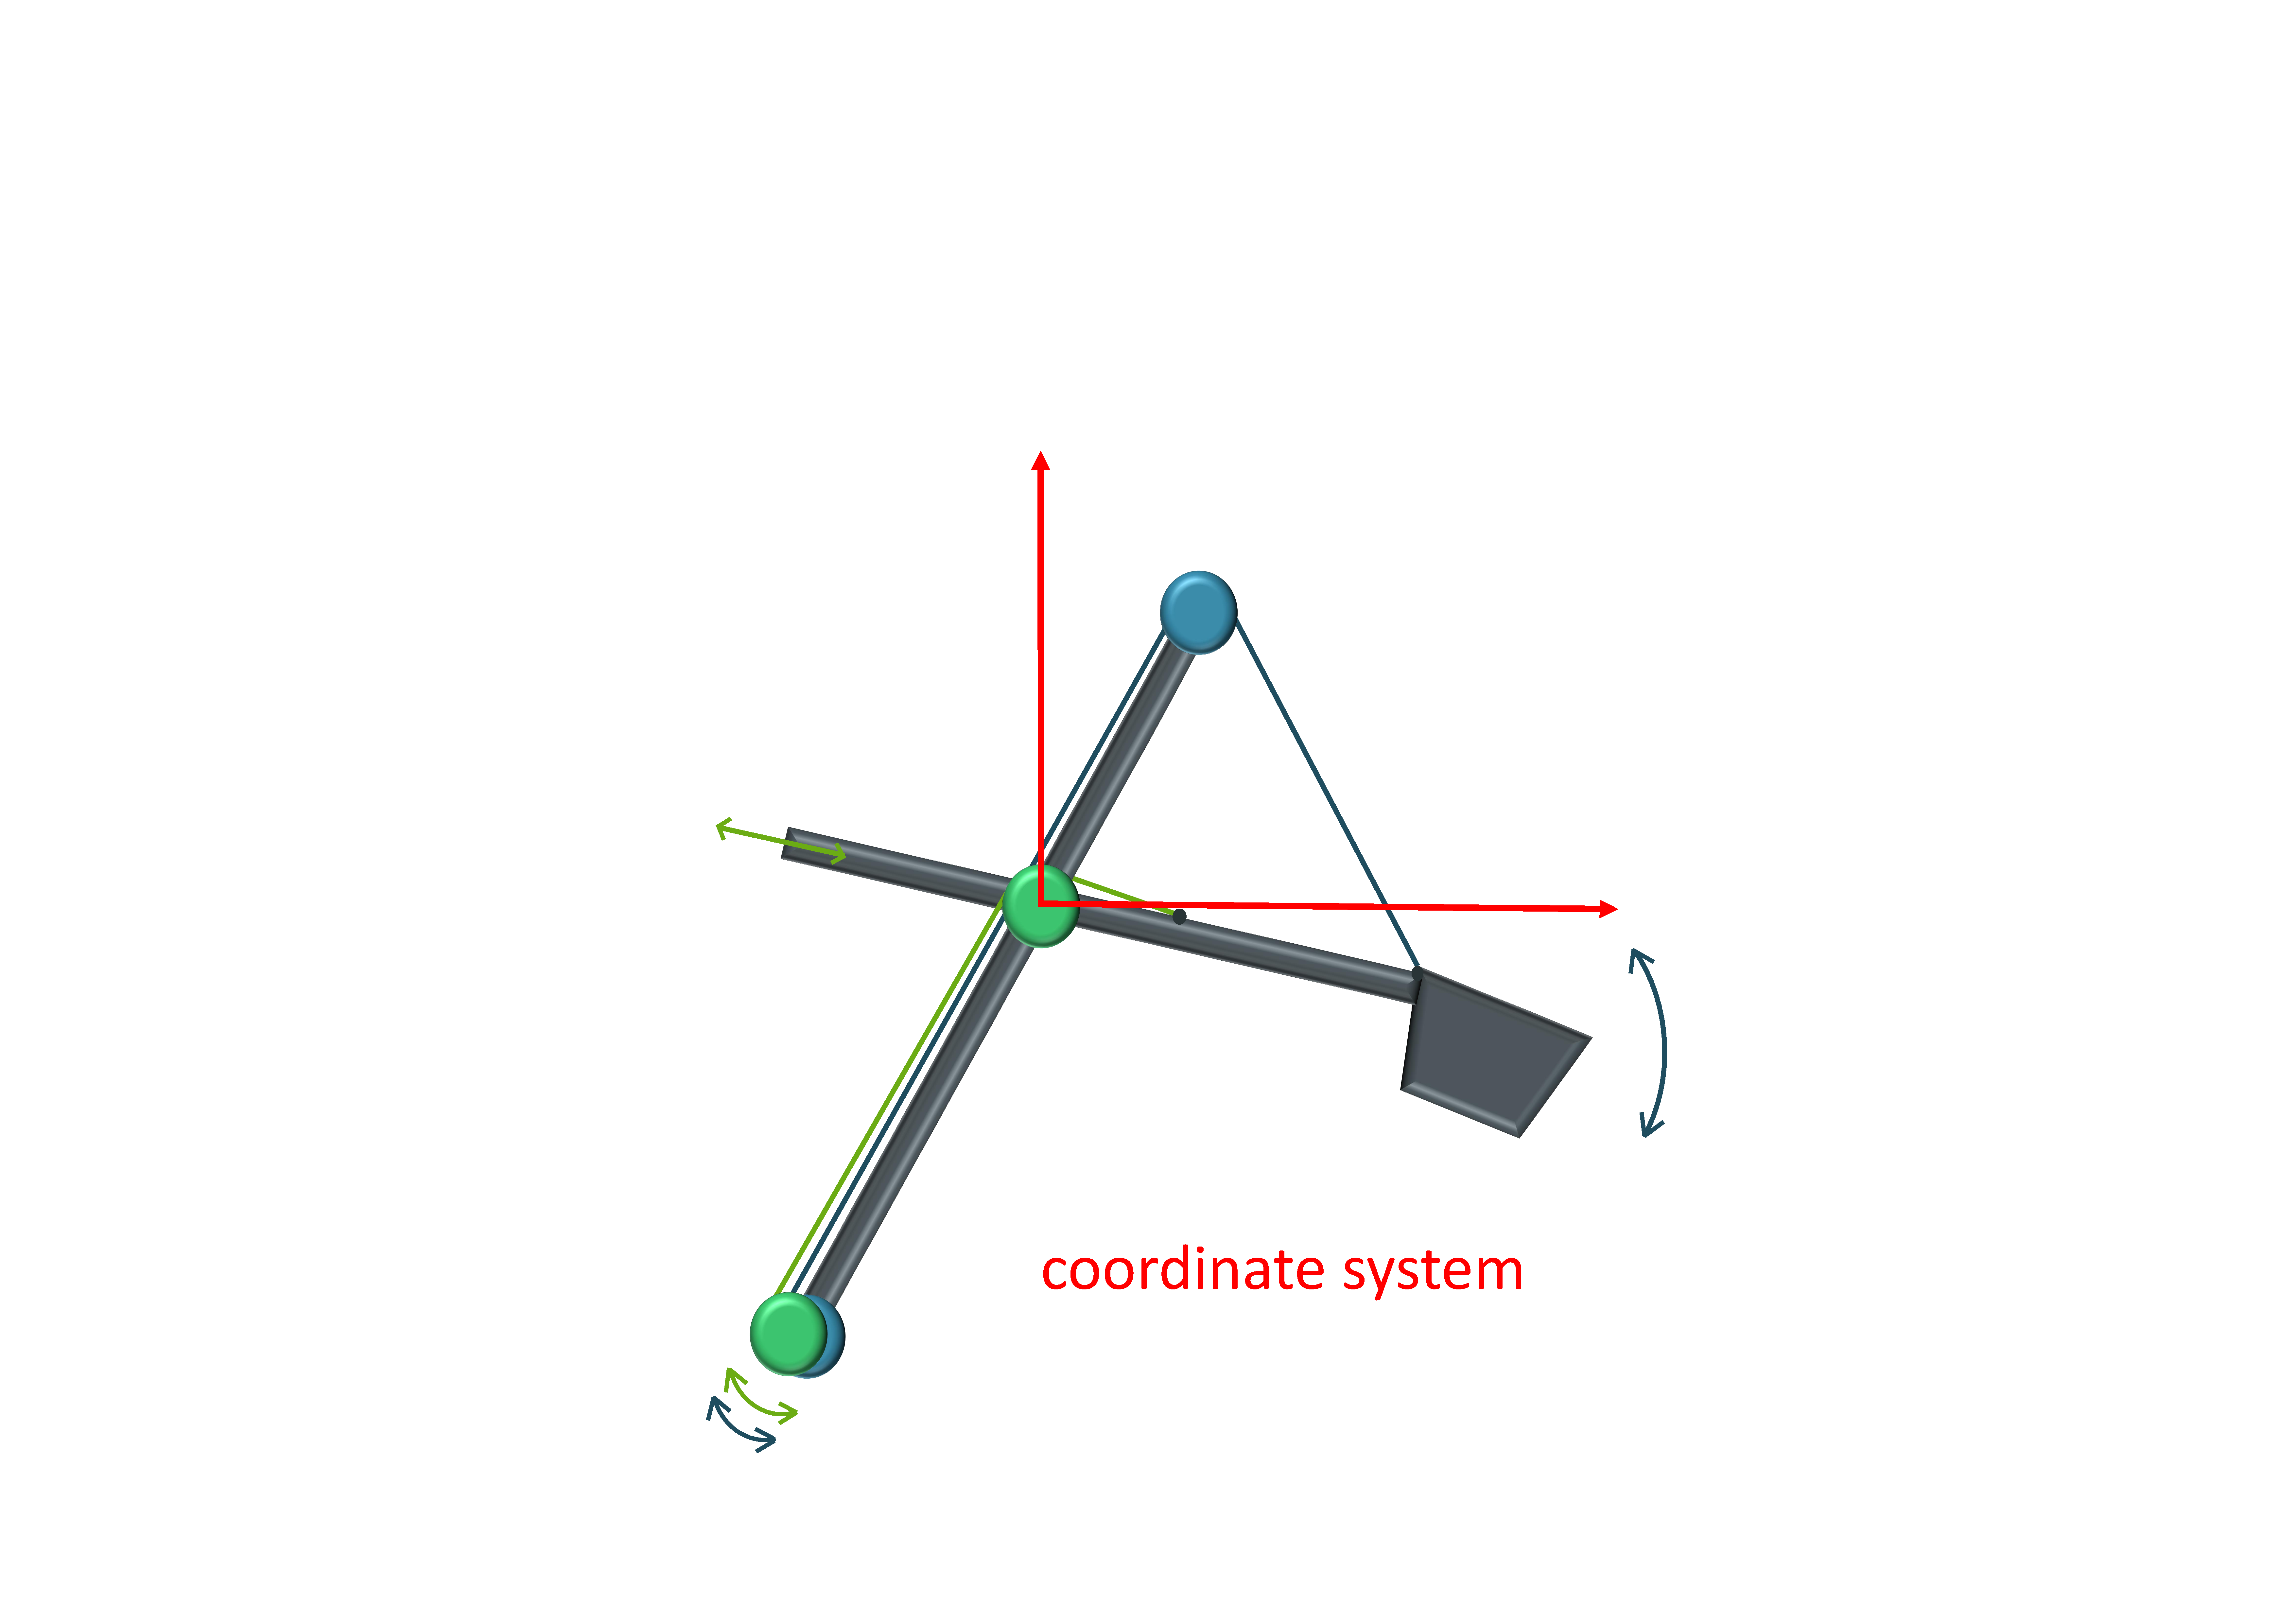
\includegraphics[trim=22cm 5cm 2cm 23cm, clip=true, width=\linewidth]{Exc/Excavator_coordinates2}
	
\end{frame}

\begin{frame}
	\frametitle{Physical Model of Excavator}
	
	%think of degrees of freedom $\rightarrow$ angle and length side arm $\rightarrow$ forces in the system will depend on excavator configuration and therefore on $s$ and $\theta$\\
	
	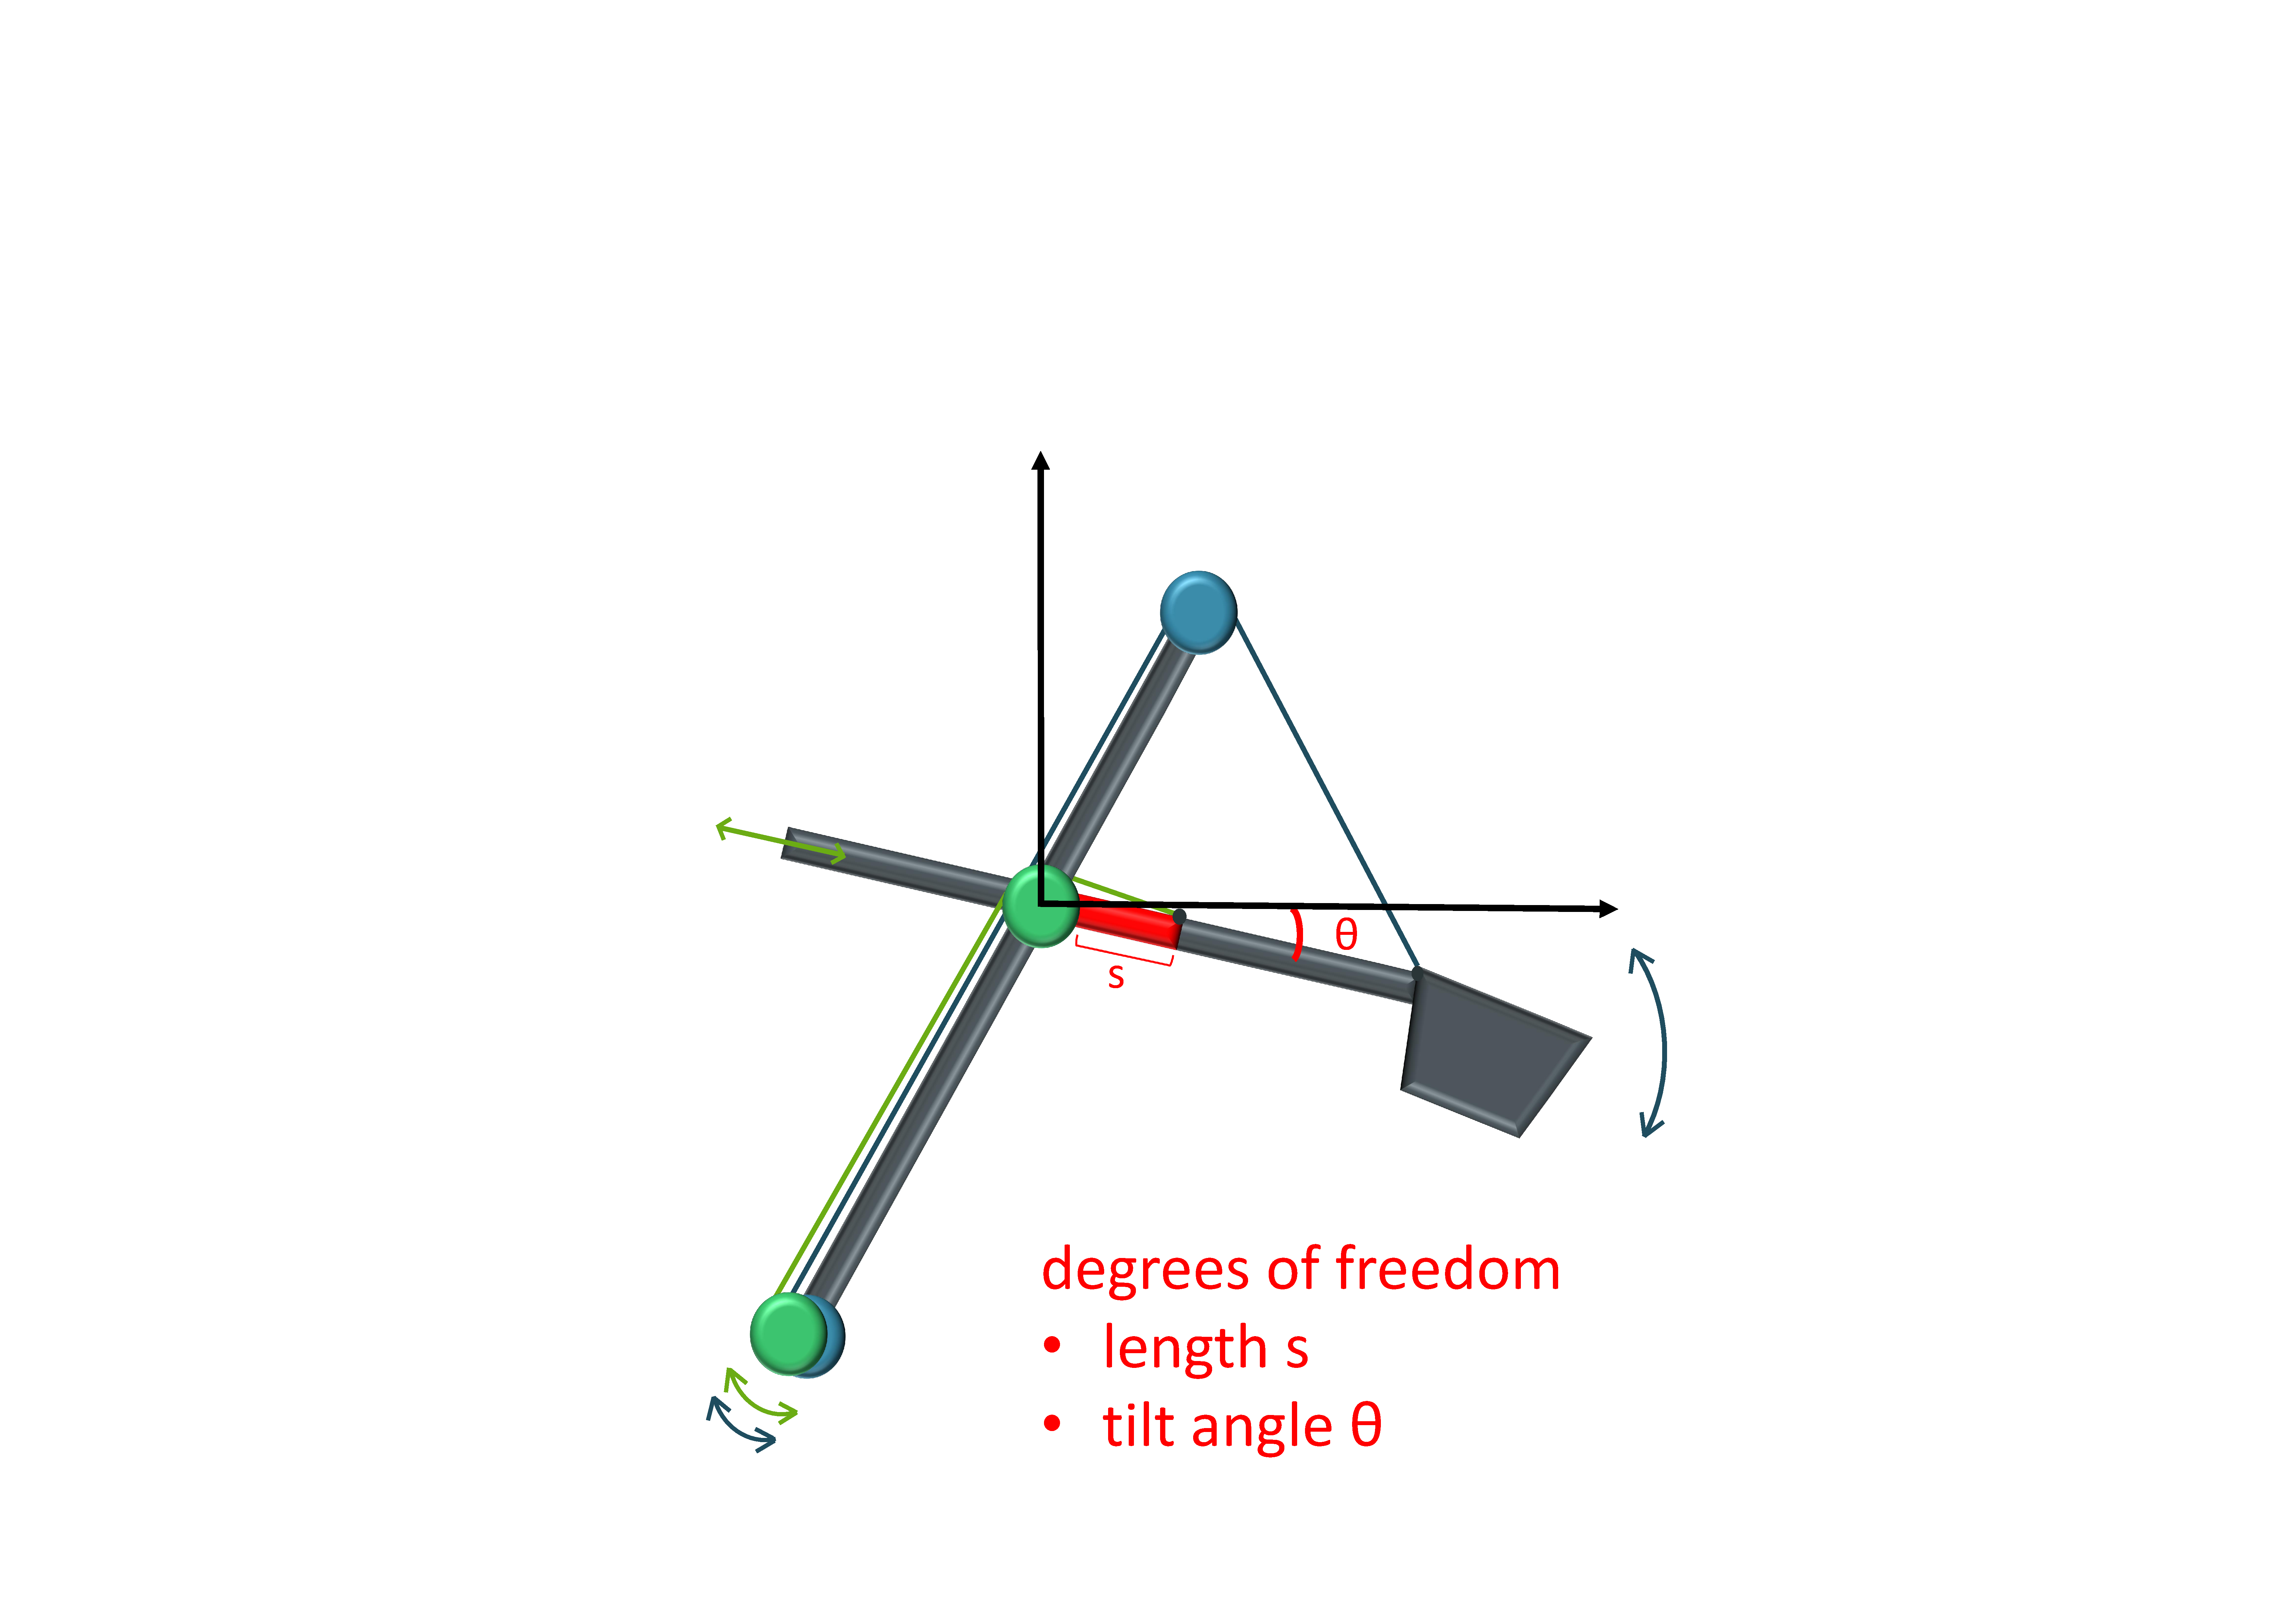
\includegraphics[trim=22cm 5cm 2cm 23cm, clip=true, width=\linewidth]{Exc/Excavator_dof2}
	
	% s distance between attachment point and upper cable reel of green pulley
	
\end{frame}

\begin{frame}
	\frametitle{Physical Model of Excavator}
	
	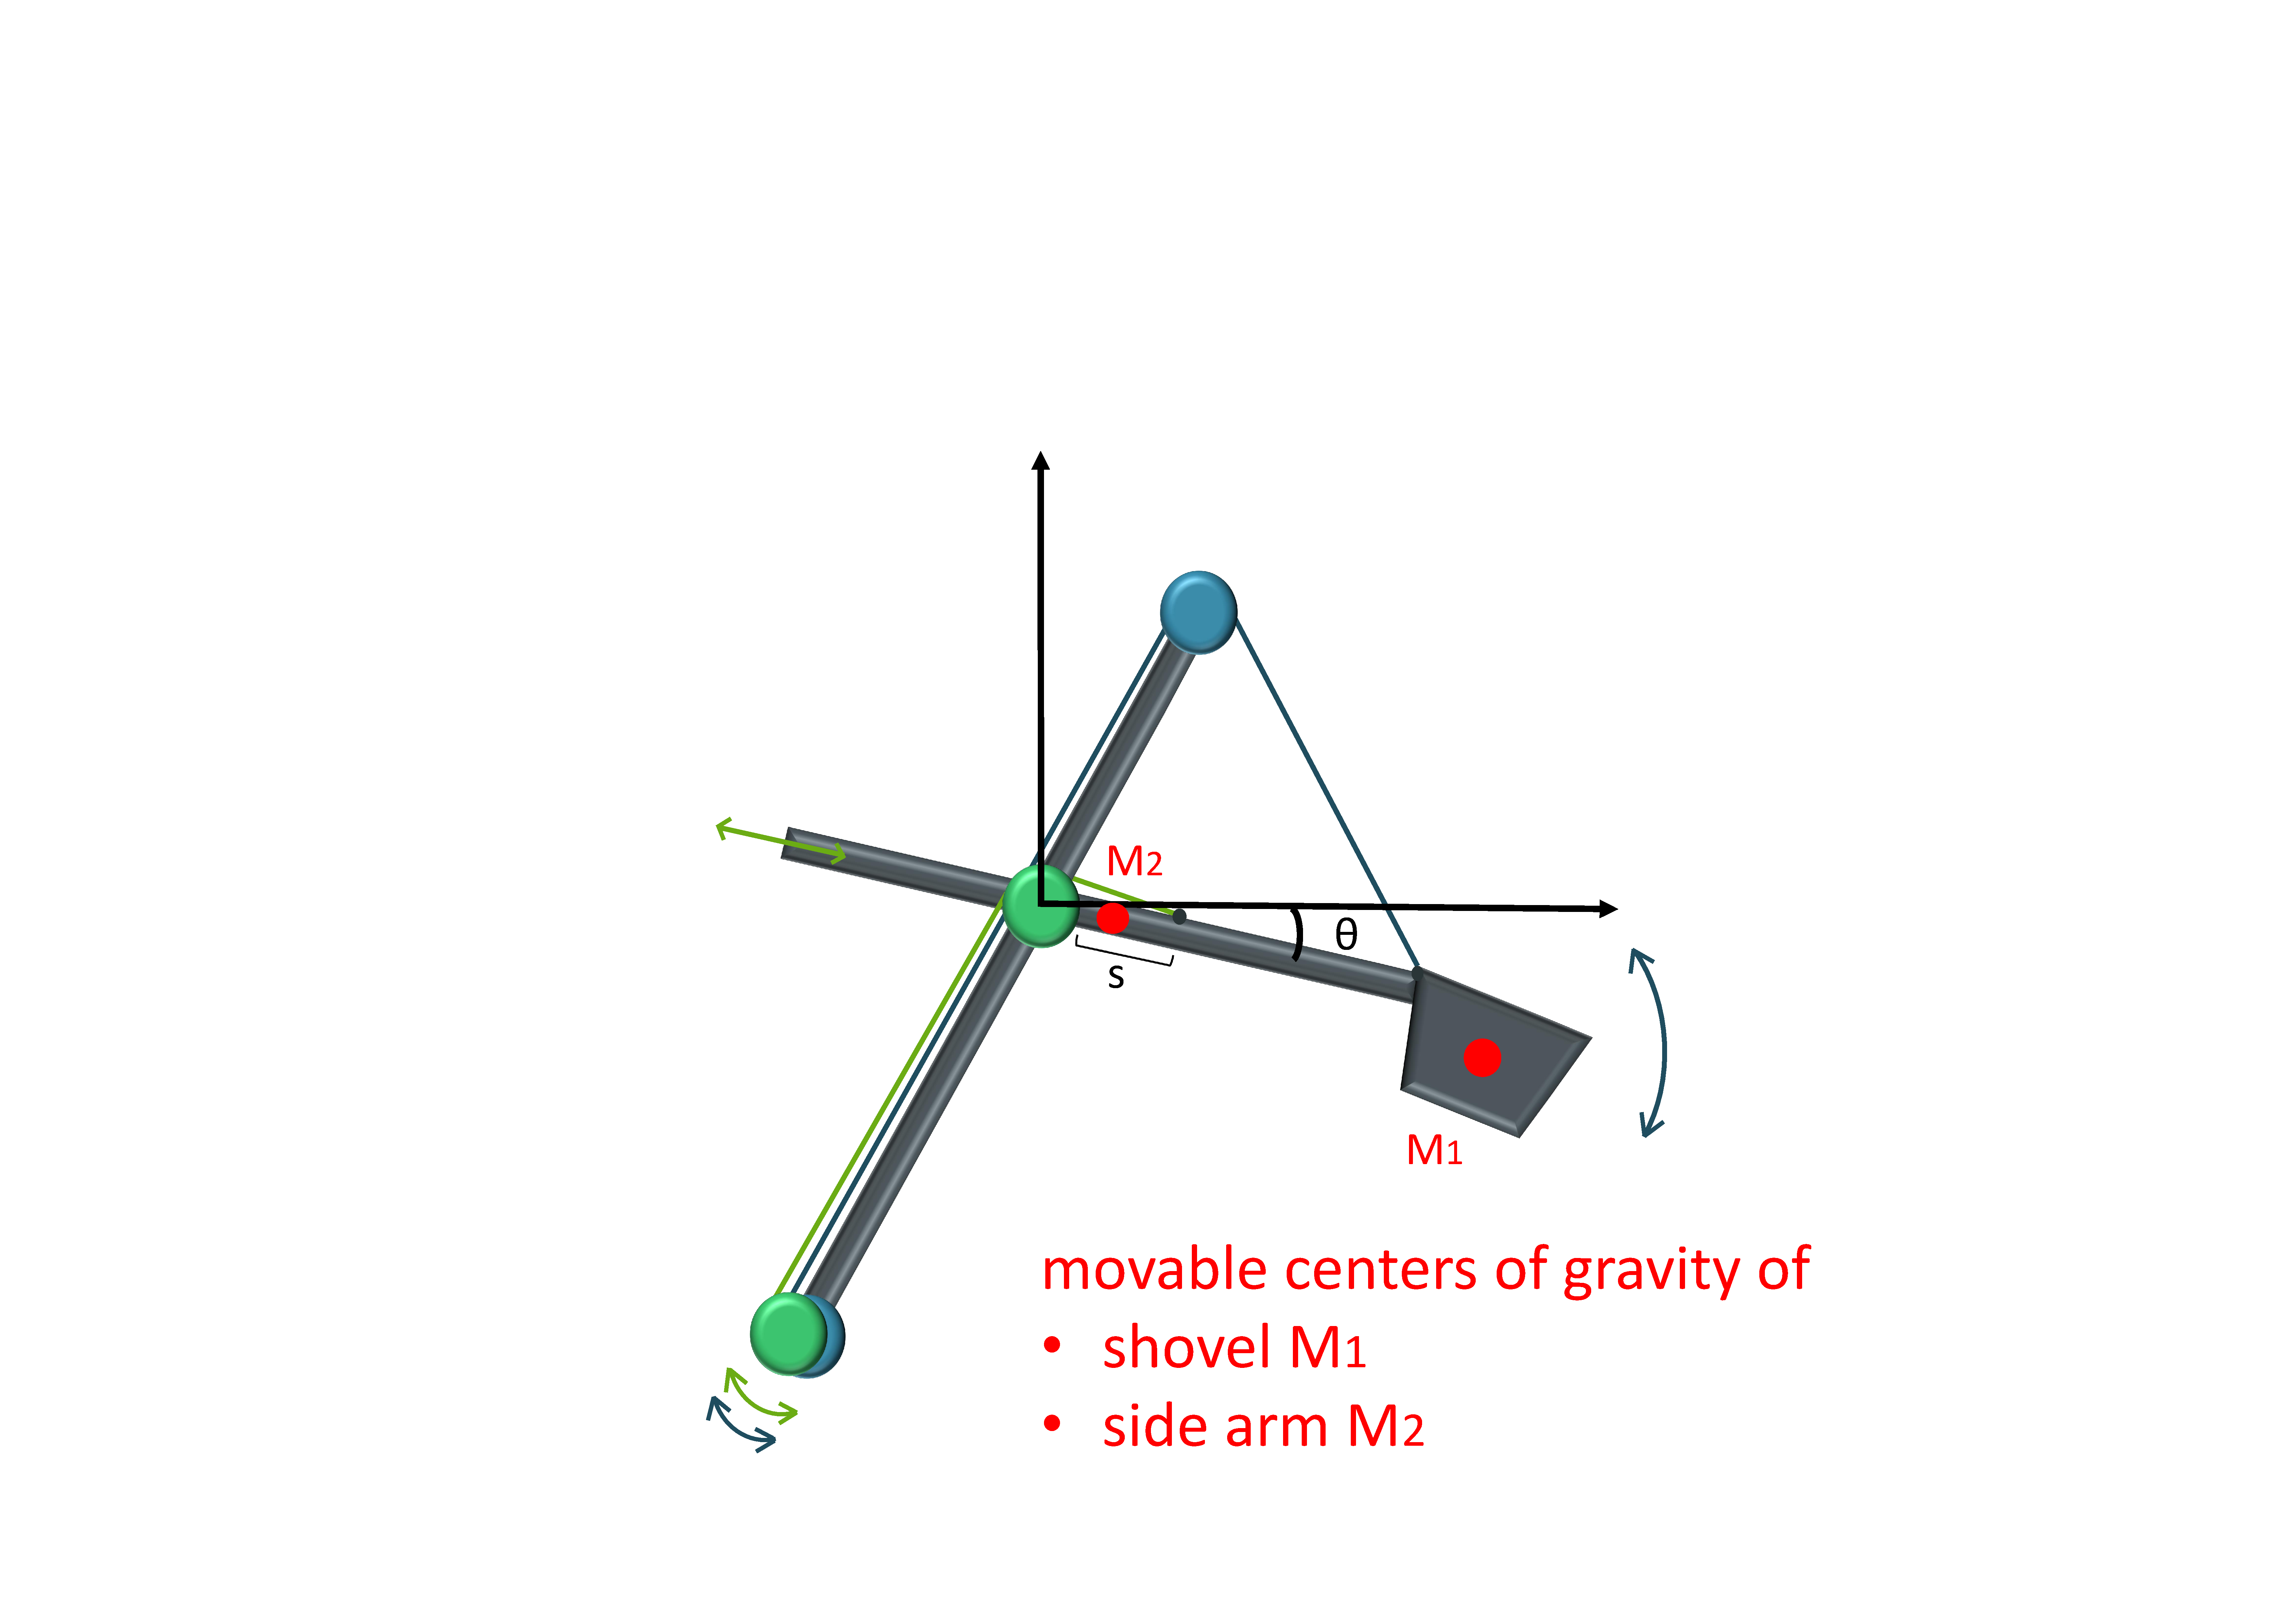
\includegraphics[trim=22cm 5cm 2cm 23cm, clip=true, width=\linewidth]{Exc/Excavator_mass2}
	
\end{frame}

\begin{frame}
	\frametitle{Physical Model of Excavator}
	
	%where are the point masses? only consider point masses which can be moved i.e. depend on configuration $\rightarrow$ derivative wrt degrees of freedom\\
	%shovel and center of mass of side arm\\
	%other arm is fixed and cant be moved
	
	Assumptions to the model:\\
	$ $ \\
	\begin{itemize}
		\item ropes do not have masses
		\item consider shovel as point mass % attached on the side arm
		\item no slack between ropes and cable reels
		% ropes and cable reel move with same velocity
		% only bearing friction (friction within cable reels)
	\end{itemize}
	
\end{frame}

\begin{frame}
	\frametitle{Kinetic Energy T}
	
	Example: energies of $M_2$ 
	\begin{align*}
		&E_{\text{kin},M_2} = \frac{1}{2}\ M_2\ \| 
		v_{O,M_2}(s,\theta,\dot{s},\dot{\theta}) \|^2 \\
		&E_{\text{rot},M_2} = \frac{1}{2}\ I_{M_2}(s)\ \dot{\theta}^2 \\
	\end{align*}
	
	all kinetic energies:
	\begin{align*}
	T\ =\ \ & E_{\text{kin},M_1} + E_{\text{kin},M_2} + E_{\text{rot},M_2}  \\
	& + E_{\text{rot},B_1} + E_{\text{rot},B_2} + E_{\text{rot},P_1} + E_{\text{rot},P_2} \\
	\end{align*}
\end{frame}

\begin{frame}
	\frametitle{Potential V}
	
	Example: potential of $M_2$
	\begin{align*}
		& V_{M_2} = M_2\ g\ h(s,\theta) \\
	\end{align*}
	
	all potentials:
	\begin{align*}
		& V = V_{M_1} + V_{M_2} \\
	\end{align*}
\end{frame}

%------------------------------------------------------------------------- Visualization ---------------------------------------------------------------------------------

\section{Visualization}

\begin{frame}[c]
	\frametitle{Visualization}
	\begin{itemize}
		\item{MatLab/Simulink}
		\vspace{0.5cm}
		\item{verification of system's behaviors by simulating the motions for characteristic inputs}
	\end{itemize}
\end{frame}

%------------------------------------------------------------------------- Parameter Optimization ------------------------------------------------------------------------

\section{Parameter Optimization}

\begin{frame}[c]
\frametitle{Parameters}
Examples:
\begin{itemize}
	\item{friction}
	\item{inertia}
	\item{mass of sidearm}
\end{itemize}
\vspace{0.5cm}
Why do we need parameter optimization?
\begin{itemize}
	\item{hard to measure}
	\item{may change over time}
\end{itemize}
\end{frame}

\begin{frame}[c]
\frametitle{Blackbox Model}
\begin{itemize}
	\item{contains a realistic model from Siemens}
	\item{content valuable}
\end{itemize}
\vspace{0.5cm}
\begin{columns}[t]
	\column{.5\textwidth}
		\textbf{Input}
		\begin{itemize}
			\item{control}
			\item{parameters}
		\end{itemize}
	\column{.5\textwidth}
		\textbf{Output}
		\begin{itemize}
			\item{motion}
		\end{itemize}
\end{columns}
\end{frame}

\begin{frame}
\frametitle{Optimization}
\begin{itemize}
	\item{no information about blackbox \\ $\Rightarrow$ derivative-free optimization}
	\vspace{0.5cm}
	\item{need own model for testing}
\end{itemize}
\end{frame}

%------------------------------------------------------------------------- Summary ---------------------------------------------------------------------------------------

\section{Summary}

\begin{frame}[c]
\frametitle{Results}
\end{frame}

\end{document}

